\chapter{Cardiac Tissue Imaging Pipeline Applications In Research}

Previous chapters have demonstrated the ability of the developed cardiac tissue clearing, mounting, and imaging protocols to be combined into a single tissue processing pipeline. This pipeline was then shown to be capable of producing high resolution images of cardiac tissue structure. The post-processing of these image stacks allows for an accurate volumetric reconstruction of the myocardium sample to be generated for use in structural analysis. Now remains two major questions that need to be answered to validate the pipeline as a technique meriting standard, general use in cardiophotonics research: 
\begin{itemize}
    \item How can this pipeline data be utilized in cardiac structural analysis? 
    \item How versatile can the pipeline data be in biological research?
\end{itemize}

This chapter will seek to answer these questions by examining three instances in which the pipeline was successfully implemented into an experimental protocol. In doing so, they showcase how this imaging data can be implemented in quantitative examination of myocardial tissue, confirming the usability and versatility of data acquired by the processing pipeline.

These biological research projects were conducted in conjunction with the University of Glasgow’s School of Cardiovascular and Metabolic Health (SCMH), which implemented the processing pipeline and utilized the mesoSPIM microscope system assembled in School of Physics and Astronomy (PH\&A). Modifications made to the tissue staining portion of pipeline allowed these projects to obtain unique image data sets from cleared cardiac tissue. 

The first project seeks to obtain volumetric data from the innervation in cardiac tissue post myocardial infarction. The second project utilized the imaging pipeline to determine the optimal combination of fluorescent stains for use in histological analysis of left ventricle (LV) samples. The third and final project seeks to examine the ability of implanted spheroids to connect with the surrounding cardiac tissue. In all three cases, desired physiological data is dependent on the preservation of volumetric tissue structure. This data is impractical to obtain in experimental set ups using traditional, two-dimensional cardiac histology methods and can be addressed through implementation of the tissue processing pipeline.


\section{Innervation of Post-MI Leporine Hearts}
This project was conducted in collaboration with Dr. Erin Boland at the School of Cardiovascular and Metabolic Health, College of Medical, Veterinary, and Life Sciences, University of Glasgow. Steps 1-5 in the tissue processing pipeline (See Figure 2.1) were conducted by Dr. Boland and myself with subsequent imaging and data post processing completed by both me, Dr. Sharika Mohanan, and Mr. Ahmed Elnageh using Fiji ImageJ and IMARIS software. 

Methodology, data, and results acquired for this project currently under peer review for subsequent publication by advisor and paper lead author Dr. Caroline Mullenbroich at time of thesis submission. 

\subsection{Experimental Concepts}
\subsubsection{\textit{Background}}
The objective of this project is to obtain both structural and electrophysiological data from leporine heart models both healthy and post MI. This data will be used to test the hypothesis that cardiac remodelling post MI will result in alterations to the myocardium innervation. Structural and functional datasets obtained from samples will be correlated to determine associations between structural formations and electrical activity in the organ. Obtaining these correlated sets of data will allow changes to the sympathetic innervation that occurs because of tissue remodelling post-myocardial infarction to be documented and analysed further in research settings [].


Currently established methods of examining sympathetic innervation in cardiac tissue provide only limited spatial and morphological detail from existing histology methods requiring tissue slices no greater than 10 microns in thickness to conduct []. It is hypothesized that the combination an optimized tissue clearing pipeline with innervation targeted labelling of cardiac tissue samples will permit faster acquisition with greater spatial resolution, simpler image reconstruction, and higher structural preservation than previously possible in established histological assessments.

\subsubsection{\textit{Methodologies}}

For this experiment, 8 leporine hearts (New Zealand White Rabbits) underwent functional data recording attached to Langendorff perfusion set up. the imaging pipeline utilizing CLARITY tissue clearing protocol (See Chapter 3) was subsequently implemented on 10 tissue slices (0.5 mm and 1.0 mm thickness) extracted from the LV wall of functional data recorded heart models. (N,total = 10; n, healthy = 3; n, scar = 7). 

\paragraph{Staining}

Samples then initially underwent staining protocols based on previously published procedures along with guidelines provided by the antibody manufacturers []. Adjustments to the protocol were implemented based on the results achieved using this base protocol with multiple concentrations and combinations of fluorescent, antibody stains. These adjustments aimed to improve florescent signal intensity, reduce background noise, and ensure sufficient and homogeneous stain penetration into the tissue volume. Stains that aim to florescence specific structures in the tissue, such as cell nuclei or tissue innervation, were also examined to ensure labelling in these channels remained specific with every adjustment made to the initial protocol. The finalized staining protocol created is described with precise timing steps with timings and volumes in Table 5.1:

\begin{table}[H]
    \centering
    \begin{tabular}{cc}
        \textbf{Procedure Step} & \textbf{Time Duration}\\
            \medskip
         1. PBS Washing & 3 Hours\\
             \medskip
         2. PBS-T Washing & 24 Hours\\
            \medskip
         3*. 1:200 Anti-TH Antibody Wash in PBS-T at $4\celsius$ & 72 Hours\\
            \medskip
         4. 1:100 WGA/AF-488 Conjugate Stain Wash & 48 Hours\\
            \medskip
         5*. 1:200 Goat anti-mouse AF 647 Secondary Antibody Wash in PBS-T & 48 Hours\\
            \medskip
         6. 1:1000 DAPI Nuclear Stain Wash in PBS-T & 6 Hours**\\
            \medskip
         6. PBS-T Wash (3x) & 8 Hours (x3)\\
            \medskip
         7. 4\% PFA/PBS Wash & 15 Min\\
            \medskip
         8. PBS Washes (x3) & 5 Min (3x)\\
            \medskip
    \end{tabular}
    \medskip
    \caption{\textbf{Finalized antibody/WGA conjugate dual staining protocol for CLARITY cleared tissue slices.} All steps performed with gentle agitation at Room Temperature (RT) unless otherwise stated. Steps 3-8 are light sensitive, performed with light shielding around sample at all times. *Antibody staining steps skipped if DAPI utilized. **DAPI can be added to last 6 hours of prior washing step, step skipped if antibody staining performed.}
    
\end{table}


After optimization of staining to the best of our ability, two 0.5mm thick, CLARITY cleared tissue slice samples were stained using two unique staining combinations Dr. Erin Boland and myself. 

The first tissue was stained with a combination of WGA/AF-488 and the nucleic acid stain DAPI, which followed the protocol presented in Table 5.1 but with the antibody staining steps omitted with nuclear dye staining steps performed in their place. The second tissue was stained with WGA/AF-488 and the antibody anti-Tyrosine hydroxylase (Anti-TH; ThermoFisher MA5-32984) following the same staining protocol with antibody staining steps intact. 

\paragraph{Image Acquisition}

Stained tissues were mounted by myself according to the imaging pipeline sliced tissue mounting procedures (see Chapter 4) and imaged according to mesoSPIM mounted sliced tissue protocols (see Chapter 2). The entire tissue volume of each sample was recorded across multiple image stack tiles stitched together using BigStitcher software package on Fiji ImageJ software \cite{horl_bigstitcher_2019}. The python script implemented for the point spread analyses of agarose bead samples in Chapter 4 was again applied to two regions of interest (ROIs) in the tissue sample stained with WGA/AF-488 and DAPI (see INSERT GITHUB URL) to analyse cell nuclei that could be discerned in the recorded and no-shear processed image of the tissue produced. 

\paragraph{Data Processing}

Image reconstruction is performed on data collected from this sample to determine if the staining protocol in combination with the greater imaging pipeline is capable of discerning the fragile and intricate fibre-like network of nerve cells, which distinguishes myocardial innervation, across the cleared tissue sample \cite{saltzman_biomedical_2015}. The qualitative examination of the reconstructed volume from the oblique scanned, no-shear processed images will determine if the process can be implemented on a larger scale to perform more quantitative analysis of the intricate remodelling of cardiac tissue innervation in post-MI tissue samples compared to non MI, healthy controls. 

Point spread analysis is performed using signal acquired from cell nuclei in the sample to validate the no shear processing method as capable of reconstructing images from oblique scans with sufficient resolution and image quality to discern, count, and calculate densities of cell nuclei across the sample. Point spread analysis process created and optimized by Mr. Ahmed Elnageh in python script (available in [GITHUB URL, folder location]). Successful completion of this quantitative analysis with results mirroring estimates for nuclei number and density expected in cardiac tissue samples is used to confirm if a given tissue is viable for use in biological histology. 




\subsection{Experimental Results}
\subsubsection{\textit{Nuclear Stain, No Shear Imaging Analysis}}

Upon completion of image processing, a full volume reconstruction of the sliced tissue was generated in the Fiji ImageJ software \cite{schindelin_fiji_2012}. The figure on the next page showcases signal acquired from DAPI and WGA-AF 488 stains within a single imaging frame, within a single frame of the reconstructed volume, approximately 0.25 mm beneath the surface of the tissue slice.

\begin{figure}[H]
\centering
\begin{subfigure}[t]{0.9\textwidth}
\includegraphics[width=1\linewidth]{Images/Fig5_1.png}
\caption{\textbf{Stitched image of 0.5 mm leporine cardiac tissue slice cleared with CLARITY and stained using WGA/AF-488 and DAPI.} Scale Bar = 5 mm. Magenta channel (405 nm), cyan channel (488 nm).}
\end{subfigure}
\medskip

\begin{subfigure}[t]{0.475\textwidth}
\centering
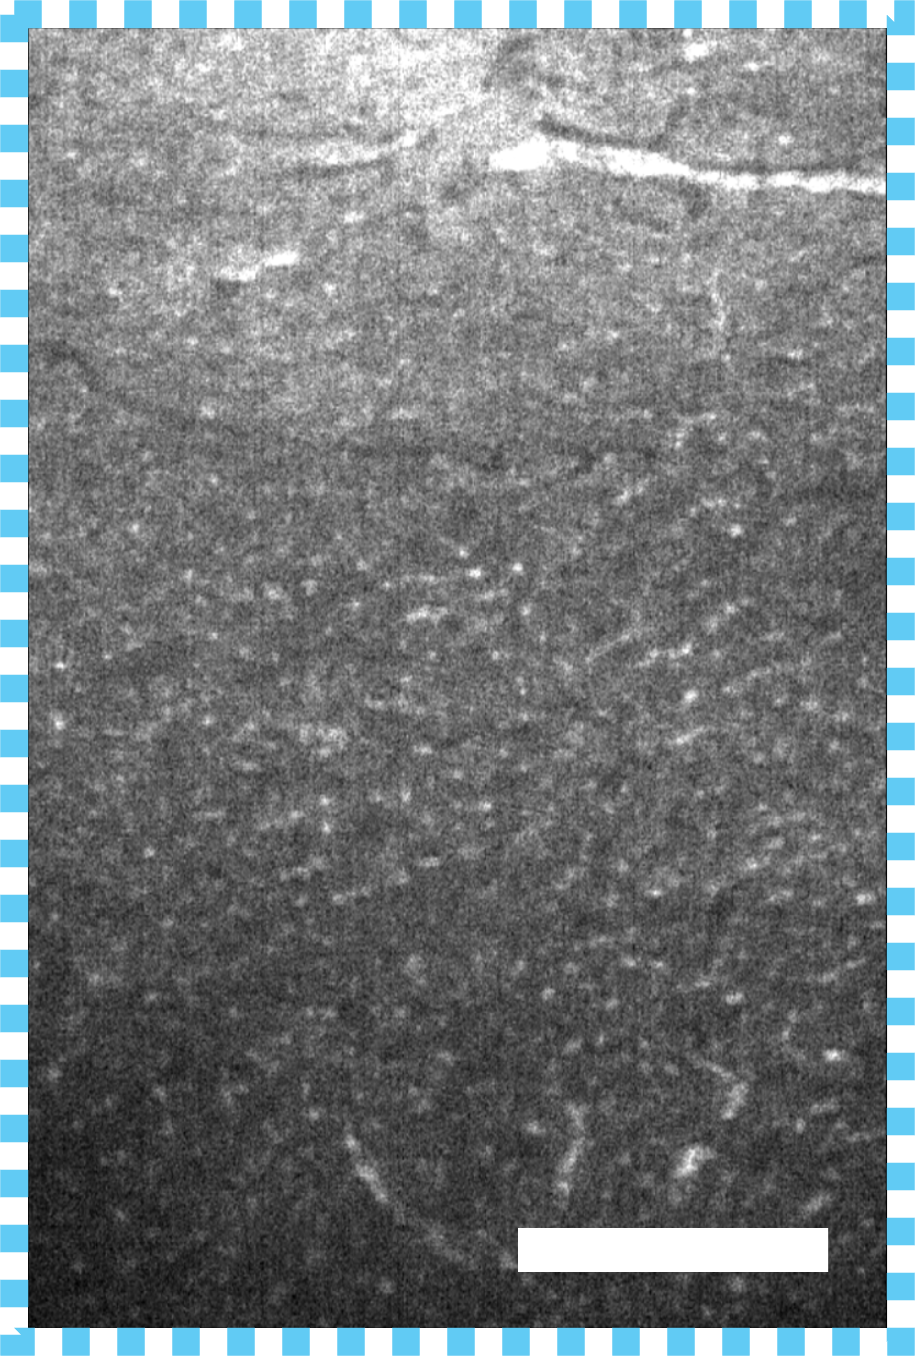
\includegraphics[width=0.75\linewidth]{Images/ROI1.png}
\caption{\textbf{ROI \#1.} Highlighted in cyan in (a), Scale Bar = 300 microns.}
\end{subfigure}
\medskip
~
\begin{subfigure}[t]{0.475\textwidth}
\centering
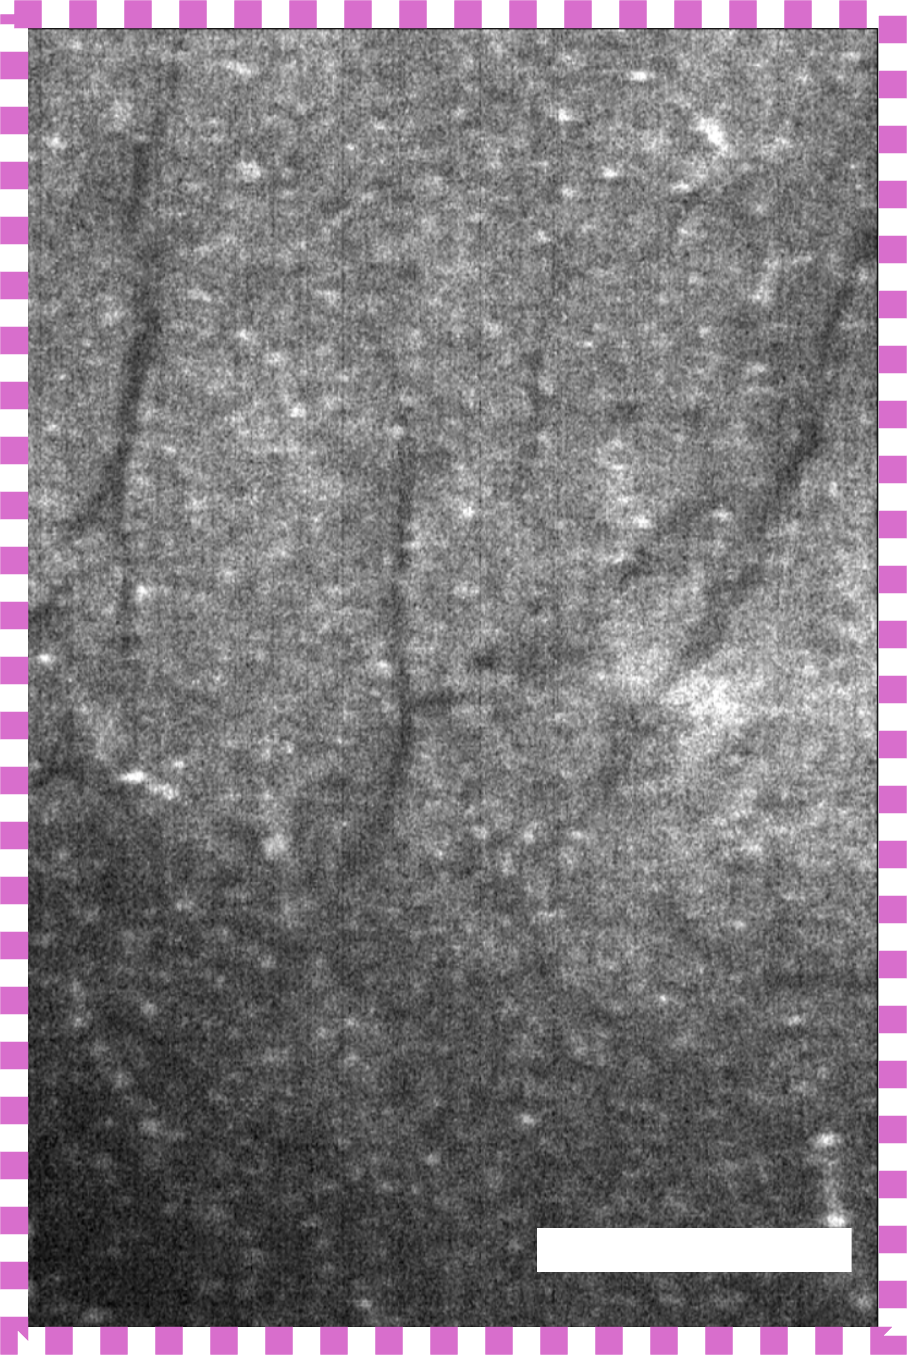
\includegraphics[width=0.75\linewidth]{Images/ROI2.png}
\caption{\textbf{ROI \#2.} Highlighted in pink in (a), Scale Bar = 300 microns.}
\end{subfigure}
\caption{\textbf{Results of no-shear image processing in combination with tissue imaging pipeline processes.} Tissue orientated at 45 degree angle with respect to detection, excitation pathways. Light sheet is orientated perpendicularly with respect to the reconstructed, de-skewed images shown above.}
\end{figure}

As seen in Figure 5.1, the no shear method of data processing in combination with the adapted dual fluorescent dye staining protocol was able to produce images of tissue structure with sufficiently high resolution and contrast to distinguish individual cell nuclei and membranes across the 0.5 mm thick cardiac tissue slice with homogenous visibility of cell nuclei located within the densely packed fibres of the myocardium. These nuclei in selected ROIs from the DAPI emission channel were measured according to the sample coordinate system (x',y ,z'; see Chapter 4.2.2) and the distribution of measurements in each axis for each ROI is shown on the following page:

\begin{figure}[H]
\centering
    \begin{subfigure}[t]{0.49\textwidth}
        \centering
        \begin{tikzpicture}
            \begin{axis}
            [
            scale = 1,
            ytick={1,2,3},
            yticklabels={Z',Y, X'},
            xlabel={Axis},
            ylabel={Recorded Bead Dimension (microns)},
            boxplot/box extend=0.25,
            xmax = 25,
            xlabel = {Length ($\mu$m)}
            ]
    
   \addplot+[boxplot, mark=none] 
            table [y index=0] {Data/ROI1/zfwhm.txt}
            [above]
            node at
              (boxplot whisker cs:\boxplotvalue{lower whisker},1)
              {\pgfmathprintnumber{\boxplotvalue{lower whisker}}}
            node at
              (boxplot box cs: \boxplotvalue{median},-1)
              {\pgfmathprintnumber{\boxplotvalue{median}}}
            node at
              (boxplot whisker cs:\boxplotvalue{upper whisker},1)
              {\pgfmathprintnumber{\boxplotvalue{upper whisker}}}
            ;
            
    \addplot+[boxplot, mark=none] 
            table [y index=0] {Data/ROI1/yfwhm.txt}
            [above]
            node at
              (boxplot whisker cs:\boxplotvalue{lower whisker},1)
              {\pgfmathprintnumber{\boxplotvalue{lower whisker}}}
            node at
              (boxplot box cs: \boxplotvalue{median},1)
              {\pgfmathprintnumber{\boxplotvalue{median}}}
            node at
              (boxplot whisker cs:\boxplotvalue{upper whisker},1)
              {\pgfmathprintnumber{\boxplotvalue{upper whisker}}}
            ;
   \addplot+[boxplot, mark=none] 
            table [y index=0] {Data/ROI1/xfwhm.txt}
            [above]
            node at
              (boxplot whisker cs:\boxplotvalue{lower whisker},1)
              {\pgfmathprintnumber{\boxplotvalue{lower whisker}}}
            node at
              (boxplot box cs: \boxplotvalue{median},-1)
              {\pgfmathprintnumber{\boxplotvalue{median}}}
            node at
              (boxplot whisker cs:\boxplotvalue{upper whisker},1)
              {\pgfmathprintnumber{\boxplotvalue{upper whisker}}}
            ;
            \end{axis}
 
        \end{tikzpicture}
        \caption{\textbf{ROI 1 (n=43)}}
    \end{subfigure}
    \medskip
    ~
    \begin{subfigure}[t]{0.49\textwidth}
        \centering
        \begin{tikzpicture}
           \begin{axis}
            [
            scale = 1,
            ytick={1,2,3},
            yticklabels={Z',Y, X'},
            boxplot/box extend=0.25,
            xmax = 25,
            xlabel = {Length ($\mu$m)}
            ]
    
   \addplot+[boxplot, mark=none] 
            table [y index=0] {Data/ROI2/zfwhm.txt}
            [above]
            node at
              (boxplot whisker cs:\boxplotvalue{lower whisker},1)
              {\pgfmathprintnumber{\boxplotvalue{lower whisker}}}
            node at
              (boxplot box cs: \boxplotvalue{median},-1)
              {\pgfmathprintnumber{\boxplotvalue{median}}}
            node at
              (boxplot whisker cs:\boxplotvalue{upper whisker},1)
              {\pgfmathprintnumber{\boxplotvalue{upper whisker}}}
            ;
            
    \addplot+[boxplot, mark=none] 
            table [y index=0] {Data/ROI2/yfwhm.txt}
            [above]
            node at
              (boxplot whisker cs:\boxplotvalue{lower whisker},1)
              {\pgfmathprintnumber{\boxplotvalue{lower whisker}}}
            node at
              (boxplot box cs: \boxplotvalue{median},-1)
              {\pgfmathprintnumber{\boxplotvalue{median}}}
            node at
              (boxplot whisker cs:\boxplotvalue{upper whisker},1)
              {\pgfmathprintnumber{\boxplotvalue{upper whisker}}}
            ;
   \addplot+[boxplot, mark=none] 
            table [y index=0] {Data/ROI2/xfwhm.txt}
            [above]
            node at
              (boxplot whisker cs:\boxplotvalue{lower whisker},1)
              {\pgfmathprintnumber{\boxplotvalue{lower whisker}}}
            node at
              (boxplot box cs: \boxplotvalue{median},-1)
              {\pgfmathprintnumber{\boxplotvalue{median}}}
            node at
              (boxplot whisker cs:\boxplotvalue{upper whisker},1)
              {\pgfmathprintnumber{\boxplotvalue{upper whisker}}}
            ;
            
            \end{axis}
        \end{tikzpicture}
        \caption{\textbf{ROI 2 (n=133)}}
    \end{subfigure}
    \caption{\textbf{Distribution of cell nuclei dimensional measurements.} Median, upper and lower quartiles, max and min extrema shown. Measurements recorded in sample coordinate system (x', y, z').}
    \label{fig:enter-label}
\end{figure}

The FWHM of cell nuclei measurements in both ROIs were compared to the resolution limits established by the agarose bead characterization experiments. The comparison in distribution of these axial dimension measurements are presented in Figure 5.3: 

\begin{figure}[H]
        \centering
        \begin{tikzpicture}
            \begin{axis}
            [
            scale = 1,
            ytick={1,2,3},
            yticklabels={$Z'_{ROI_2}$,$Z'_{ROI_1}$,\empty},
            xlabel={Axis},
            ylabel={Recorded Bead Dimension (microns)},
            boxplot/box extend=0.25,
            xmin= 6,
            xmax = 18, 
            ymin = 0,
            ymax=3,
            xlabel = {Length ($\mu$m)}
            ]
    
     \addplot+[boxplot, mark=none] 
            table [y index=0] {Data/ROI2/zfwhm.txt}
            [above]
            node at
              (boxplot box cs: \boxplotvalue{median},1.1)
              {\pgfmathprintnumber{\boxplotvalue{median}}}
            ;
    \addplot+ [boxplot prepared={lower whisker=13.23, upper whisker=13.23,whisker extend = 4,draw position=1,every whisker/.style={magenta,ultra thick}}] 
                %table [y index=0] {Data/double/zfwhm.txt}
                coordinates {};
                    %;
    \addplot+ [boxplot prepared={lower whisker=7.76, upper whisker=7.76,whisker extend = 4,draw position=1,every whisker/.style={cyan,ultra thick}}]
                %table [y index=0] {Data/double/zfwhm.txt}
                coordinates {};
                    %;
    \addplot+[boxplot, mark=none] 
            table [y index=0] {Data/ROI1/zfwhm.txt}
            [above]
            node at
              (boxplot box cs: \boxplotvalue{median},1.1)
              {\pgfmathprintnumber{\boxplotvalue{median}}}
            ;
              \end{axis}
        \end{tikzpicture}
        \caption{\textbf{FWHM distribution of cell nuclei axial measurements in ROIs (Fig. 5.1(a-b)).} (N, ROI \#1 = 27 nuclei; N, ROI \#2 = 132 nuclei)  Median axial measurement, inner quartiles, minimum and maximum values are shown. magenta line = shear imaging method axial resolution limit (13.23 microns). Cyan line = no shear method axial resolution limit (7.76 microns).}
    \end{figure}

It was seen in this comparison of axial data that the resolution required to properly discern cell nuclei in the axial dimension is higher than the average resolution limit established in characterization tests for sliced sample mounting using the shear technique. The majority of nuclei in ROI \#1 (Fig. 5.1(b)) could be discerned by the shear method, including the second through fourth quartiles of nuclei recorded. In ROI \#2, however, only the fourth and upper half of the third quartile of recorded nuclei could have been resolved as the remainder of nuclei in the ROI were out of the shear method's axial resolution range. This is in stark contrast to the no-shear method's axial resolution limit, which was capable of resolving a larger range of cell nuclei sizes, which in the myocardium can span from 5 to 15 microns in width []. With only a small number of nuclei recorded falling below the no-shear resolution limit in ROI \#2, and the inner quartiles of recorded nuclei in both ROIs falling well above the resolution limit, the application of the no shear technique was considered successful in identifying and measuring the general population of cell nuclei in cardiac tissue processed and imaged through the imaging pipeline.

\subsubsection{\textit{Anti-TH Immunolabelling, No Shear Imaging Analysis}}

For the tissue sample stained utilizing WGA/AF-488 and anti-TH antibody immunostaining, the volume of the tissue sample was reconstructed utilizing BigStitcher software programme on Fiji ImageJ \cite{horl_bigstitcher_2019}. Anti-TH immunostaining will target the neuronal structural contained within the sample and the images recorded, emitting the highest level of signal in those regions of the sample in which the innervation of the myocardium remains intact. The following figure showcases signal acquired from the Anti-TH and WGA/AF-488 stains within a section of the reconstructed volume containing the highest density regions of signal seen from the anti-TH channel.  

\begin{figure}[H]
    \centering
    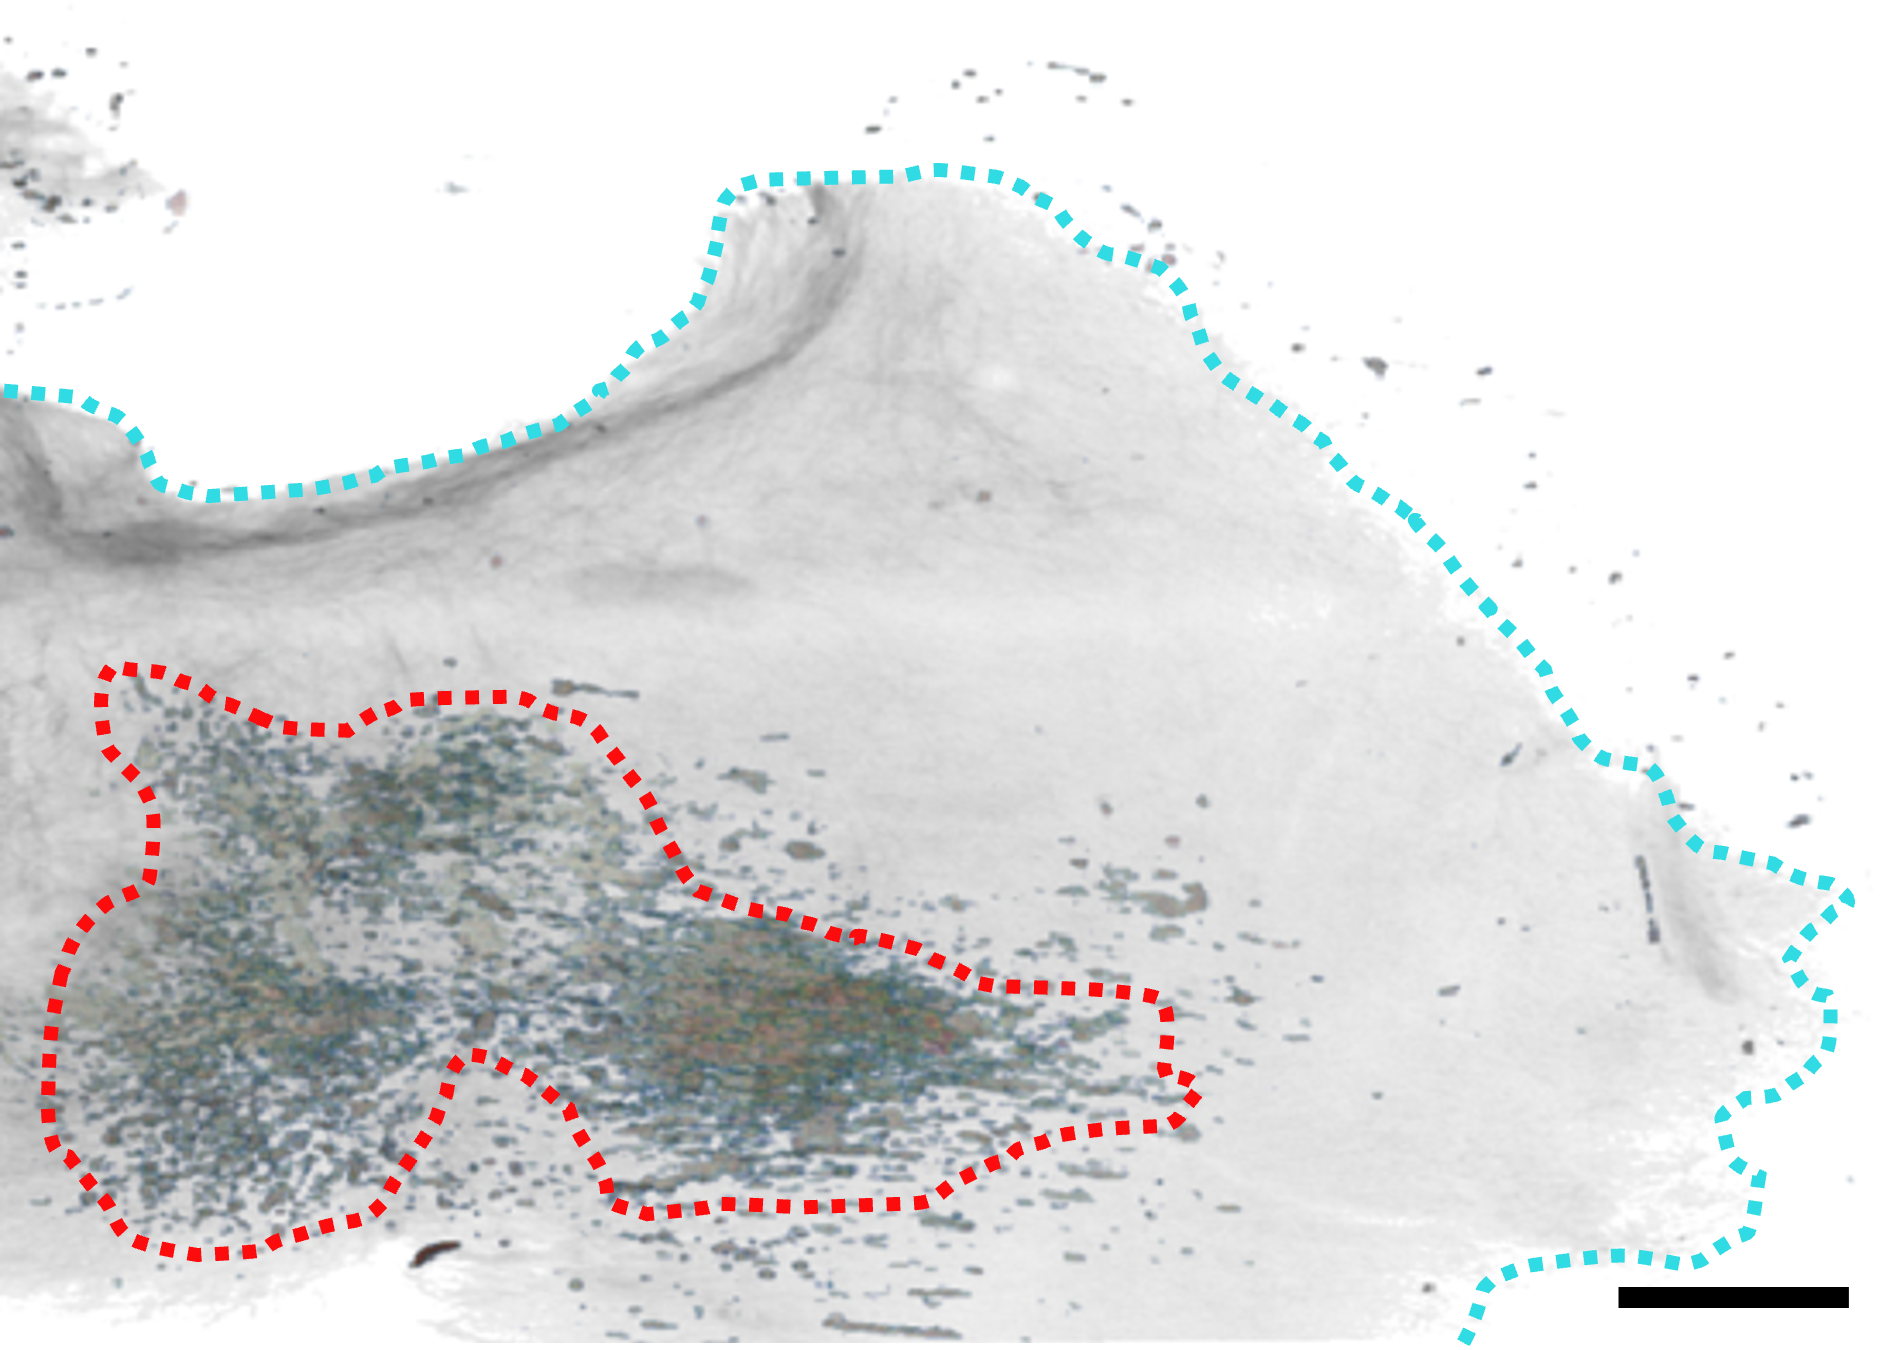
\includegraphics[width=1\linewidth]{Images/Anti_TH_Overview2.png}
    \caption{\textbf{Overview image frame of 0.5 mm leporine cardiac tissue slice cleared with CLARITY and stained using WGA/AF-488, Anti-TH Antibody Staining.} Scale bar = 1000 microns. 647 and 488 excitation channels overlaid, colour-inverted using Fiji ImageJ Software. Cyan dotted line marks boundary of tissue volume fluoresced by WGA/AF-488, Red dotted line marks boundary of tissue volume densely fluoresced by anti-TH. Light sheet is orientated perpendicularly with respect to the reconstructed imaging planes shown above.}
\end{figure}
\medskip

 The individual image channels for WGA/AF-488 and Anti-TH is provided in Figure 5.5. Select ROIs, for zoomed in looks at cell morphological details visible in each channel, are also provided besides the images of their respective imaging channels of origin.

\begin{figure}[H]
    \begin{subfigure}[t]{0.5\textwidth}
    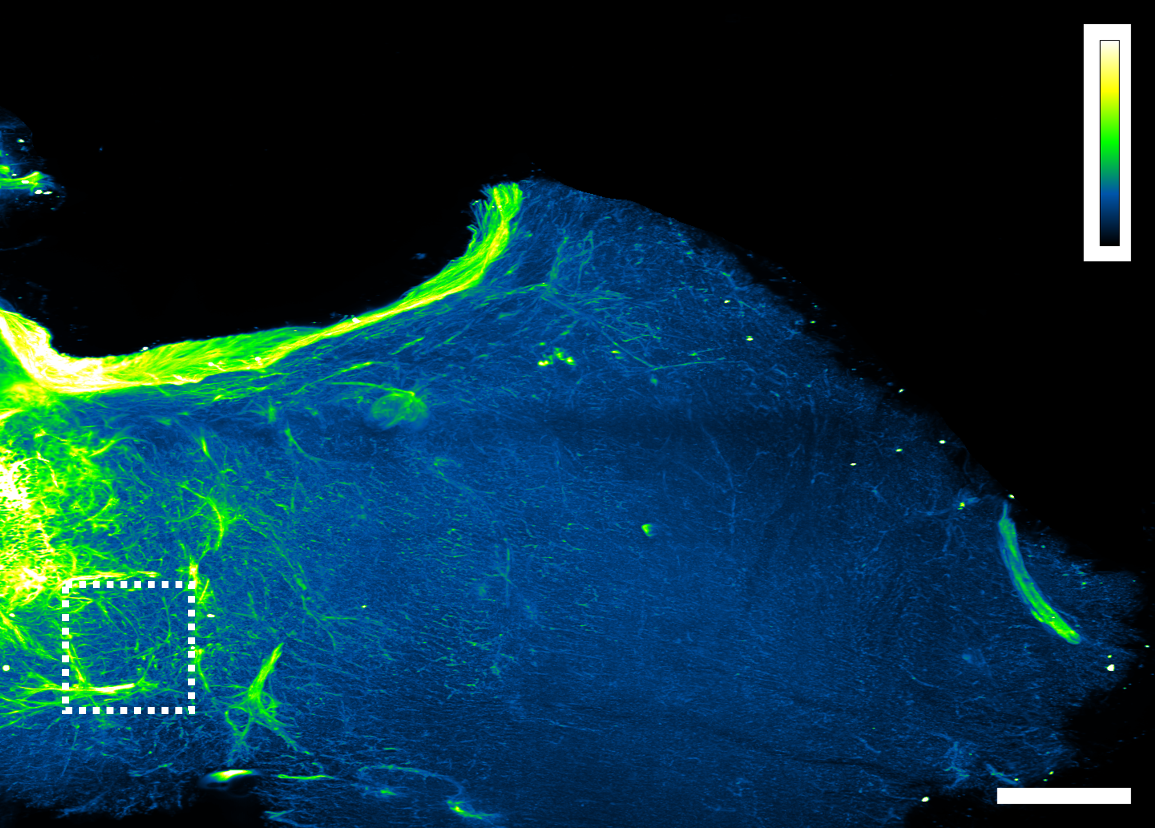
\includegraphics[width=1\linewidth]{Images/wga_channel.png}
    \caption{\textbf{WGA/AF-488 channel of image frame.} Scale bar = 1000 microns.}
    \end{subfigure}
    \medskip
    ~
    \begin{subfigure}[t]{0.45\textwidth}
    \centering
    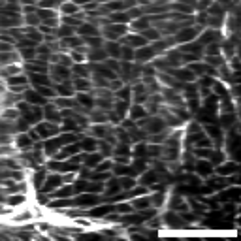
\includegraphics[width=0.8\linewidth]{Images/wga_zoomin.png}
    \caption{\textbf{ROI \#1 (Highlighted in white in (a)).} Scale bar = 250 microns.}
    \end{subfigure}
    \medskip
    
    \begin{subfigure}[t]{0.5\textwidth}
    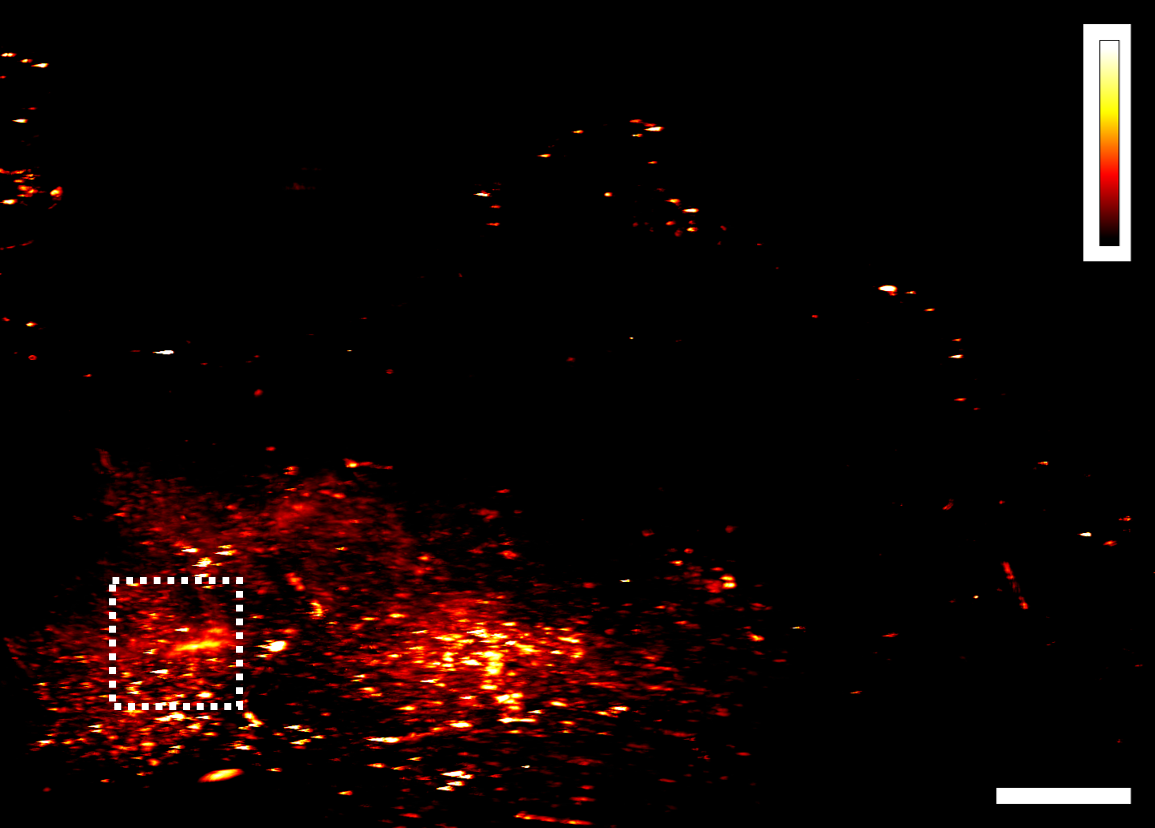
\includegraphics[width=1\linewidth]{Images/anti_Th_channel.png}
    \caption{\textbf{Anti-TH channel of image frame.} Scale bar = 1000 microns.}
    \end{subfigure}
    \medskip
    ~
    \begin{subfigure}[t]{0.45\textwidth}
    \centering
    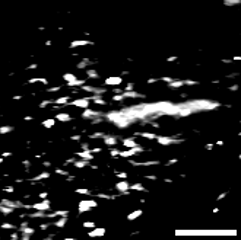
\includegraphics[width=0.8\linewidth]{Images/anti_th_zoomin.png}
    \caption{\textbf{ROI \#1 (Highlighted in white in (c)).} Scale bar = 250 microns.}
    \end{subfigure}
    \medskip
    
\caption{\textbf{Individual channels and zoomed in ROIs of 0.5 mm leporine cardiac tissue slice cleared with CLARITY and stained using WGA/AF-488, anti-TH antibody staining.} Image processing performed by Dr. Sharika Mohanan. Signal intensity (value: 0 (yellow) - 255 (red/blue)). Profiles in yellow-blue (WGA/AF-488) and yellow-red (anti-TH). Light sheet is orientated perpendicularly with respect to the imaging planes shown above.}
\end{figure}

3D reconstructions of the innervation pathways seen in selected ROIs across the images tissue volume were assembled and are shown on the next page (Fig. 5.6(b-c)) with colour highlights marking the ROI locations in the Anti-TH Overview Image (Fig 5.6(a)).

\begin{figure}[H]
    \centering
    \begin{subfigure}[t]{0.6\textwidth}
    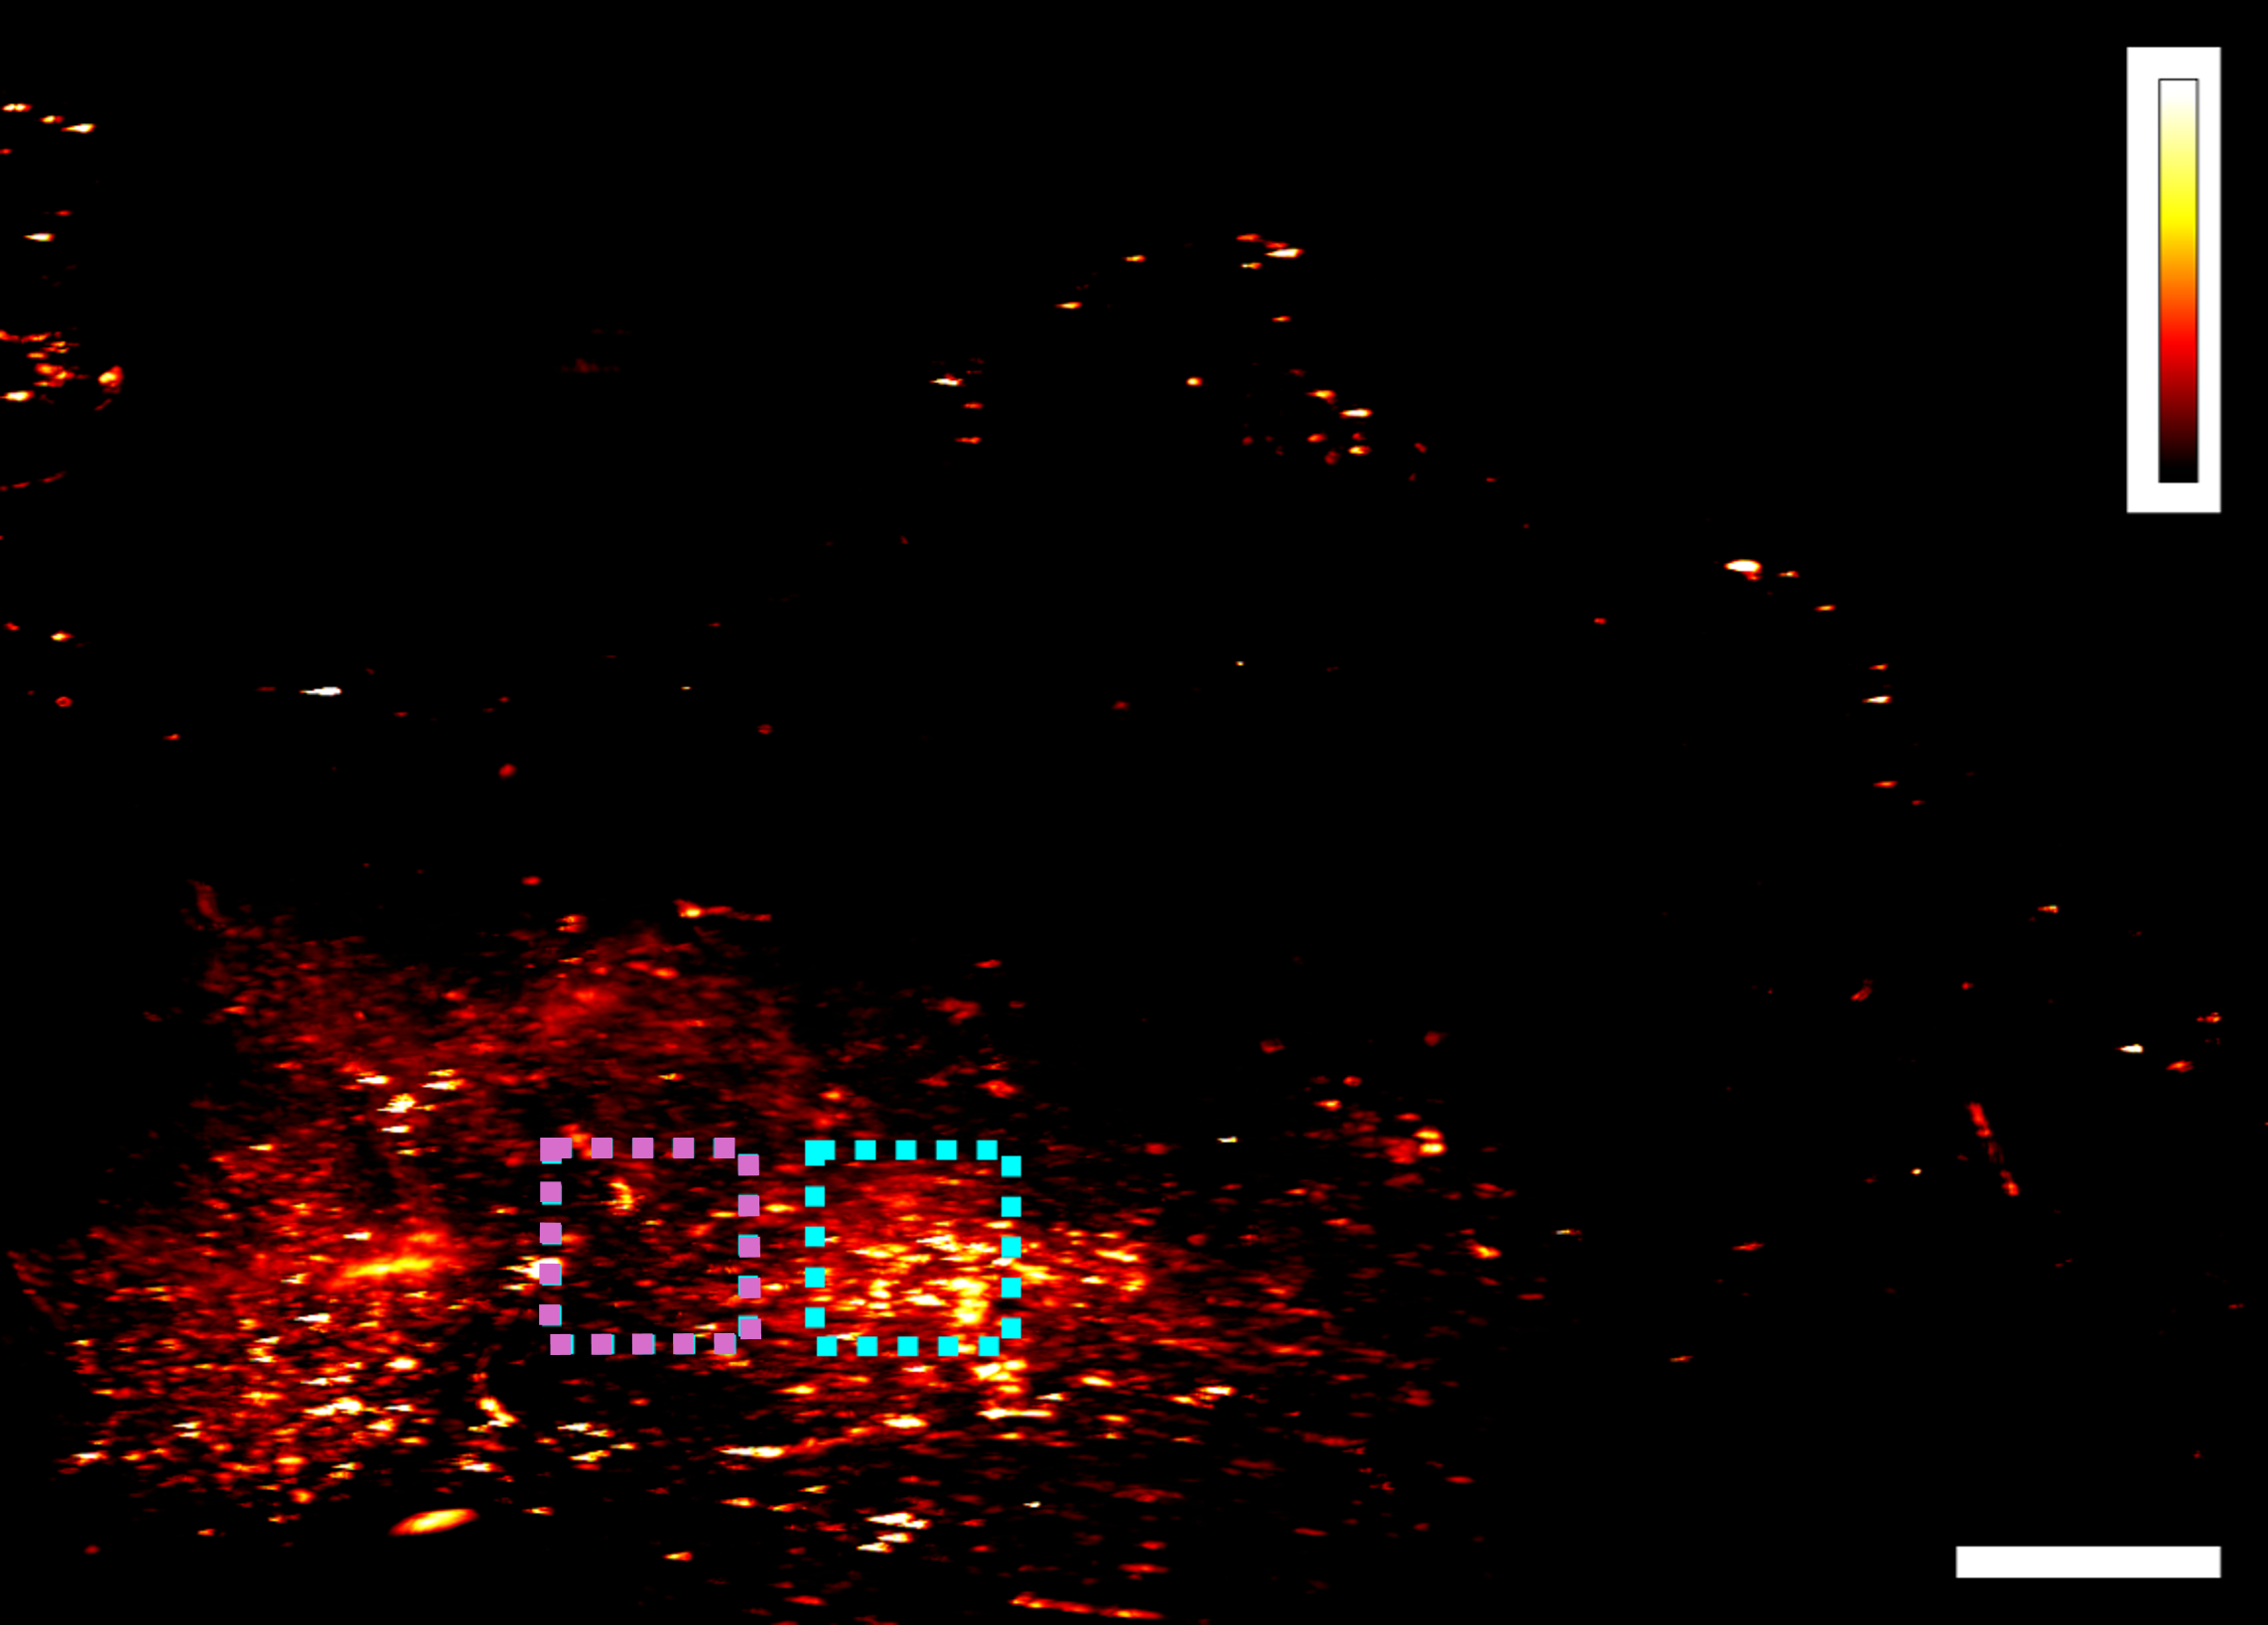
\includegraphics[width=1\linewidth]{Images/antith_roi_overview.png}
    \caption{\textbf{Anti-TH channel of image frame.} Scale bar = 50 micron. Signal intensity profiles in yellow-red (anti-TH); Signal intensity (value: 0 (yellow) - 255 (red))}
    \end{subfigure}
    \medskip
    
    \begin{subfigure}[f]{0.475\textwidth}
    \centering
    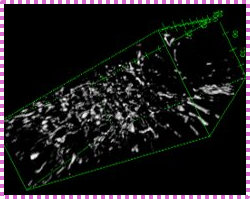
\includegraphics[width=1\linewidth]{Images/antith_roi1.png}
    \caption{\textbf{Digital reconstruction of anti-TH signal in ROI \#2 (highlighted in magenta in (a)).}}
    \end{subfigure}
    \medskip
    ~
    \begin{subfigure}[g]{0.475\textwidth}
    \centering
    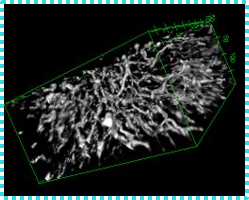
\includegraphics[width=1\linewidth]{Images/antith_roi2.png}
    \caption{\textbf{Digital reconstruction of anti-TH signal in ROI \#4 (highlighted in cyan in (a))}.}
    \end{subfigure}
    \medskip
    
    \caption{\textbf{Results 3D reconstruction of innervation pathways within select ROIs of anti-TH channel of 0.5 mm leporine cardiac tissue slices cleared with CLARITY and stained using WGA/AF-488, anti-TH antibody staining.} Image processing performed By Dr. Sharika Mohanan.}
\end{figure}


\subsection{Application Discussion}
\subsubsection{\textit{No Shear Imaging, Membrane and Nuclear Stain Discussion}}
Based on the results obtained from data collected from the nuclear and membrane stained sliced tissue samples, we confirmed that the imaging pipeline was capable of producing images and data viable for use in structural analysis of the cardiac tissue when combined with the appropriate staining protocol and image processing. No shear processing provided images of sufficient contrast and resolution to identify the individual cell membranes and nuclei that permeate the dense network of fibres that make up the myocardium (Fig 5.1 (b) and 5.4 (c)). Measured dimensions for cell nuclei was a close match to the known dimensions of cardiomyocyte and fibroblast nuclei, which range from 5 to 15 microns and have an oblong, oval shape rather than spherical as seen in agarose bead samples imaged in prior characterization tests (see Chapter 4) \cite{woodcock_cardiomyocytes_2005}. 

Looking more closely at the axial resolution of this no shear data set, the comparison to the resolution data collected from shear process data made it clear that the improvement in resolution afforded by the no shear method is essential for the segmentation of a high percentage of nuclei in a given volume. This is made apparent by the wider distribution of axial measured nuclei's FWHM, which fails to surpass or only just approaches the axial resolution limit calculated for the shear methods of image processing (13.23 microns). This is in contrast to the no shear axially measured nuclei, whose FWHM possesses less variability and entirely surpasses the calculated axial resolution limit of the no shear method (7.75 microns). This illustrates that the no shear image processing technique is crucial to being able to compare the morphology of cardiac tissue before and after MI alterations utilizing cell nuclei segmentation. For the system to be able to discern and accurately measure the subcellular structures of the tissue sample, such as cell innervation and nuclei, the images acquired must be sufficiently visible in the axial dimension to prevent crucial details from being obscured or blurred beyond recognition. To that end, we see that only data acquired by the no shear method is capable of achieving this result.

\subsubsection{\textit{No Shear Imaging, Membrane and Anti-TH Immunolabelling Discussion}}
As opposed to the nuclear and membrane stained CLARITY cleared tissue slice imaged in this experiment series, which was quantitatively analysed, the cleared tissue slice stained in the cell membranes and innervation was examined only qualitatively. Due to the uneven staining achieved by the antibody stain, likely a result of inefficiencies with the staining process leaving the sample only stained with the expected high concentrations  of innervation in small clustered regions across the sample volume. As such, the primary goal for the images acquired for this stained sample was solely to prove that the data acquired through the no shear process could permit the digital reconstruction of the finely detailed and intricate innervation pathways that permeate the myocardial tissue slice. This includes the nerve terminals and sympathetic fibres that make up these pathways and must be distinguishable in the reconstructed volume from the rest of the pathway components for proper visual analysis of the pathway structure. 

As the mapping of functional activity over structural features in the myocardium requires these details in the innervation pathways to be present in acquired images, the ability of the no shear method to achieve this when implemented as part of the imaging pipeline supports its continued application and optimization to reconstruct the entire innervation network within cardiac samples. Sympathetic nerves of myocardial tissue experience massive alterations in cardiac tissue post MI, including the introduction of hyper-innervated and denervated regions \cite{huethorst_development_2022}. As seen in Figure 5.6(b), the three dimensional, intricate, and interconnected regions of anti-TH signal is of sufficient quality across the depth of the tissue slice to allow measurement of nerve fibre orientation, sympathetic nerve cell density, and regional innervation variations to be performed and compared to isolate those changes to innervation brought upon by an MI and to what extent these changes are (or will) become arrhythmogenic. 

Quantitative correlation of structural data obtained can from this point on be made using data acquired from existing histology methods as the control, comparison data set. Confirmation of the reliability and accuracy of data obtained from cardiac samples using the imaging pipeline is the next major step towards the wider adaption of the pipeline in research.



\section{Visualization of Structural Differences Between Leporine MI Heart Models}

This project was conducted in collaboration with Dr. Eline Huethorst at the School of Cardiovascular and Metabolic Health, College of Medical, Veterinary, and Life Sciences, University of Glasgow. Steps 1-5 in the tissue processing pipeline were conducted by Dr. Huethorst with subsequent imaging conducted by myself with Dr. Huethorst assisting. Data post processing completed by both myself and Mr. Ahmed Elnageh using Fiji ImageJ and IMARIS software \cite{schindelin_fiji_2012, rridscr_007370_imaris_nodate}. 


\subsection{Experimental Concepts}
\subsubsection{\textit{Background}}

Existing thoracotomy methods of inducing MIs in leporine models required intensive surgical procedures to halt the flow of blood into regions of LV via ligation of coronary arteries on the epicardial surface of the heart. While this method is effective in creating regions of infracted tissue for examination in cardiovascular study, the process results in the formation of additional epicardial damage (termed 'adhesions') that would not exist in naturally occurring MI events \cite{connors_postoperative_2007, freeman_novel_2024}. 

These adhesions can have detrimental effects on the imaging process and subsequent image analysis, potentially obscuring alterations to the cardiac structure due to post-MI remodelling \cite{connors_postoperative_2007}. Discerning which alterations are a result of the MI, which are a result of the thoracotomy induced adhesions, and which are a result of both is a highly subjective and time consuming process. The epicardial adhesions can also have negative impact on the ability of light sheet systems to image across the cardiac tissue with adhesions on the epicardial surface bending and scattering light from the excitation light source in unpredictable ways, preventing effective light sheet illumination of the tissue beneath the epicardium. 

To mitigate these imaging and analysis issues introduced by the thoracotomy procedure, a new percutaneous MI-model has been introduced. This method utilizes the percutaneous occlusion of coronary artery to induce MI in the left ventricle of the organ \cite{freeman_novel_2024}. By avoiding the excision of the chest and extraction of the heart from the pericardium seen in the thoracotomy method, the amount of excess tissue damage separate from the MI is considerably reduced. 

It is hypothesized that the combination of an optimized tissue clearing pipeline with membrane and nuclear targeted labelling of cardiac tissue samples will be capable of imaging samples that have undergone either method and highlight the differences in tissue structure seen between thoracotomy and percutaneous MI-models. To do this, it must be shown that the imaging protocol in combination with a dual fluorescent stain combination is capable of producing high resolution images viable for use in nuclei density and orientation calculations in heart models that have undergone either method.

\subsubsection{\textit{Methodologies}}

To begin, dual fluorescent stain combinations (one general stain and one cell nuclei specific stain) must be tested in cleared cardiac LV sections to confirm viability for imaging. These tests will confirm if a given staining combination can sufficiently penetrate and fluoresce the healthy and scarred tissue regions of samples for use in image analysis. These tests will also serve to further optimize the staining protocol created and adjusted for use in antibody staining in the previous innervation experiments. Fluorophore combinations used in this experiment, along with their respective emission and excitation peaks, are provided in appendix D.

To stain the membranes of cells within the cardiac tissue, two combinations of dual cell membrane and cell nuclei staining were utilized. The first combination included Wheat Germ Agglutinin conjugated Alexa Flour 488 (WGA-AF 488) and Propidium Iodide (PI). The second combination utilized included Wheat Germ Agglutinin conjugated Alexa Flour 647 (WGA-AF 647) and SYTOX Green. 

Each nuclear stains had excitation peaks that were distinct from their respective membrane stains and could be produced by the 488 nm, 532 nm , and 647 nm laser lines installed into the mesoSPIM laser engine. In addition to the  nuclear and membrane stain, every sample was also stained with DAPI, which could serve as an alternative nuclear stain should these yet to be optimized, primary nuclear stains (SYTOX Green, PI) produce images of poor contrast and/or resolution. 

To stain these CUBIC-L immersed samples, the finalized staining protocol created for Innervation Staining Histology experiments (See Chapter 5, Section 1) was modified to better accommodate the larger volumes of tissue contained in these cleared, LV sections. Publications and literature released by CUBICStars, developers of the CUBIC-L/RA clearing process, were implemented into the initial staining procedure (see Table 5.1) to obtain the best staining possible within these cardiac samples \cite{sands_its_2022, ueda_cubic_nodate, noauthor_cubic_nodate}. The final protocol is provided in Table 5.2:

\begin{table}[H]
    \begin{tabular}{cc}
        \textbf{Procedure Step} & \textbf{Time Duration}\\
            \medskip
         1. PBS Washing & 3 Hours\\
             \medskip
         2. PBS-T Wash (3x) & 8 Hours (x3)\\
            \medskip
         3. WGA Conjugate*, Nuclear** Stains Multiple Stain Wash & 132 Hours\\
            \medskip
         4. Continue Multiple Stain Wash at $4\celsius$ & 12 Hours\\
            \medskip
         5. PBS-T Wash (3x) at $4\celsius$ & 8 Hours (x3)\\
            \medskip
         6. PFA/PBS Wash at $4\celsius$ & 24 Hours\\
            \medskip
         7. PBS Washes (x3) & 2 Hours (3x)\\
            \medskip
         8. Incubation In 50\% CUBIC-RA Aqueous Solution & 12 Hours\\
            \medskip
         9. Incubation In 100\% CUBIC-RA Solution & $\geq 96$ Hours\\
            \medskip
    \end{tabular}
    \medskip
    \caption{\textbf{Finalized DAPI/Nuclear/WGA conjugate staining protocol for CUBIC-L/RA Cleared LV Sections.} *Compatible WGA Conjugates (1:100): WGA/AF-488, WGA/AF-555, WGA/AF-647. **Compatible Nuclear Stains: SYTOX GREEN (1:2500), PI (3:400), DAPI (1:1000). All steps performed with gentle stirring at room temperature unless otherwise stated. DAPI staining can be omitted to make double staining protocol without change to steps or time duration.}
    \label{tab:placeholder}
\end{table}


The combination staining of WGA-AF 488/PI and WGA-AF 647/SYTOX Green were applied to 4 sets of leporine left ventricle, CUBIC-L/RA cleared sections of cardiac tissue. Each set consists of 2 adjacent sections of the left ventricle wall from the same specimen, one from the left side (L) of the ventricle wall and one from the right side (R). Each sample was cleared and prepared for imaging following the established CUBIC-L/RA form of the imaging pipeline. Of these 4 specimens, 2 underwent Thoracotomy MI procedures to induce infarct via vessel ligation (1 sham, 1 real) while 2 underwent Percutaneous MI procedures (1 sham, 1 real) as previously described in Chapter 2, Section 1.1. Sham procedures serve as the controls in which the thoracotomy and percutaneous procedures are performed but the MI inducing steps of ligation or occlusion are omitted. All 4 L samples were stained using WGA-AF 647/SYTOX Green while all 4 R samples were stained using WGA-AF 488/PI. Table 5.2 below details the 8 combination of MI methods, membrane/nuclear staining, and sample location in vivo examined in this sample series.

\begin{table}[H]
    \centering
    \begin{tabular}{ccc}
         \empty & Left Side of LV Wall & Right Side of LV Wall \\
         \medskip
         \empty & WGA-AF 647/SYTOX Green & WGA-AF 488/ PI\\
         \medskip
        Percutaneous Sham & AE0D P Sham L & AE0D P Sham R\\
         \medskip
        Percutaneous MI & 2265 P MI L & 2265 P MI R\\
         \medskip
        Thoracotomy Sham & 38E2 T Sham L & 38E2 T Sham R\\
         \medskip
        Thoracotomy MI & 37D9 T MI L & 37D9 T MI R\\
         \medskip
    \end{tabular}

    \caption{\textbf{LV tissue section series imaged via imaging pipeline.} Specific leporine models indicated by unique 4 character alphanumeric code. Code combined with abbreviations as convention for sample naming (P = Percutaneous, T = Thoracotomy, L = Left, R = Right, MI = Scarred Tissue, Sham = Healthy Control Tissue).}
    \label{tab:placeholder}
\end{table}
Imaging was conducted in line with the mesoSPIM Imaging protocol for LV Sections (described in Chapter 2.3) and subsequently converted and stitched using IMARIS post processing protocols (Chapter 2.4) for use in qualitative analysis. 5\% agarose gelatine bed was added behind samples to hold in place inside the cuvette should the sample axial be found to be less than 5 mm after completing CUBIC-RA immersion.

\subsection{Experimental Results}
Imaging was performed on all 8 LV sections in the 488 nm channel along with either the 532 nm or 647 nm channels (depending on which combination of stains was used in a given sample). Due to the poor resolution observed in the DAPI channel, no imaging data was recorded and the stain was considered to be unviable in combination with the CUBIC-L/RA variation of the imaging pipeline. This was attributed to the significant increase in light scattering seen in CUBIC-L/RA tissues at lower wavelengths (see Figure 3.12) such as the 405 nm excitation light sheet used to detect DAPI emission.

\subsubsection{\textit{Qualitative Analysis of Tissue Imaging in LV Sham Thoracotomy Sample}}
Imaging data was saved onto NAS drives for subsequent processing and examination. To demonstrate that the tissue clearing pipeline (in combination with the staining process established) was capable of producing volumetric images of sufficient quality to merit further quantitative analysis, data post-processing procedure was performed on the image data sets obtained from sample 38E2 T Sham R. This included full conversion of all image tiles into IMS file format, the stitching of tiles into single image stack containing the entire tissue volume, and the conversion of stitched images back to TIFF file format utilizing the IMARIS software. Thereafter, the converted TIFF stitched images of each channel images were examined, overlaid over one another, contrast adjusted, and had maximum intensity projections (MIPs) generated of utilizing FIJI imageJ software. To examine the change in quality, if any, of imaging at varying tissue depths, MIP images were acquired from two different tissue depths in the processed tissue data (total tissue depth, $Z_{max}$ = 6003 nm): 750 microns (\~12.5\% total tissue depth) and 3000 microns (\~50\% total tissue depth). Images acquired from the light sheet positioned 750 microns deep into the LV section tissue volume are showcased in Figures 5.7-8. 


\begin{figure}[H]
    \centering
    \begin{subfigure}[t]{0.48\textwidth}
        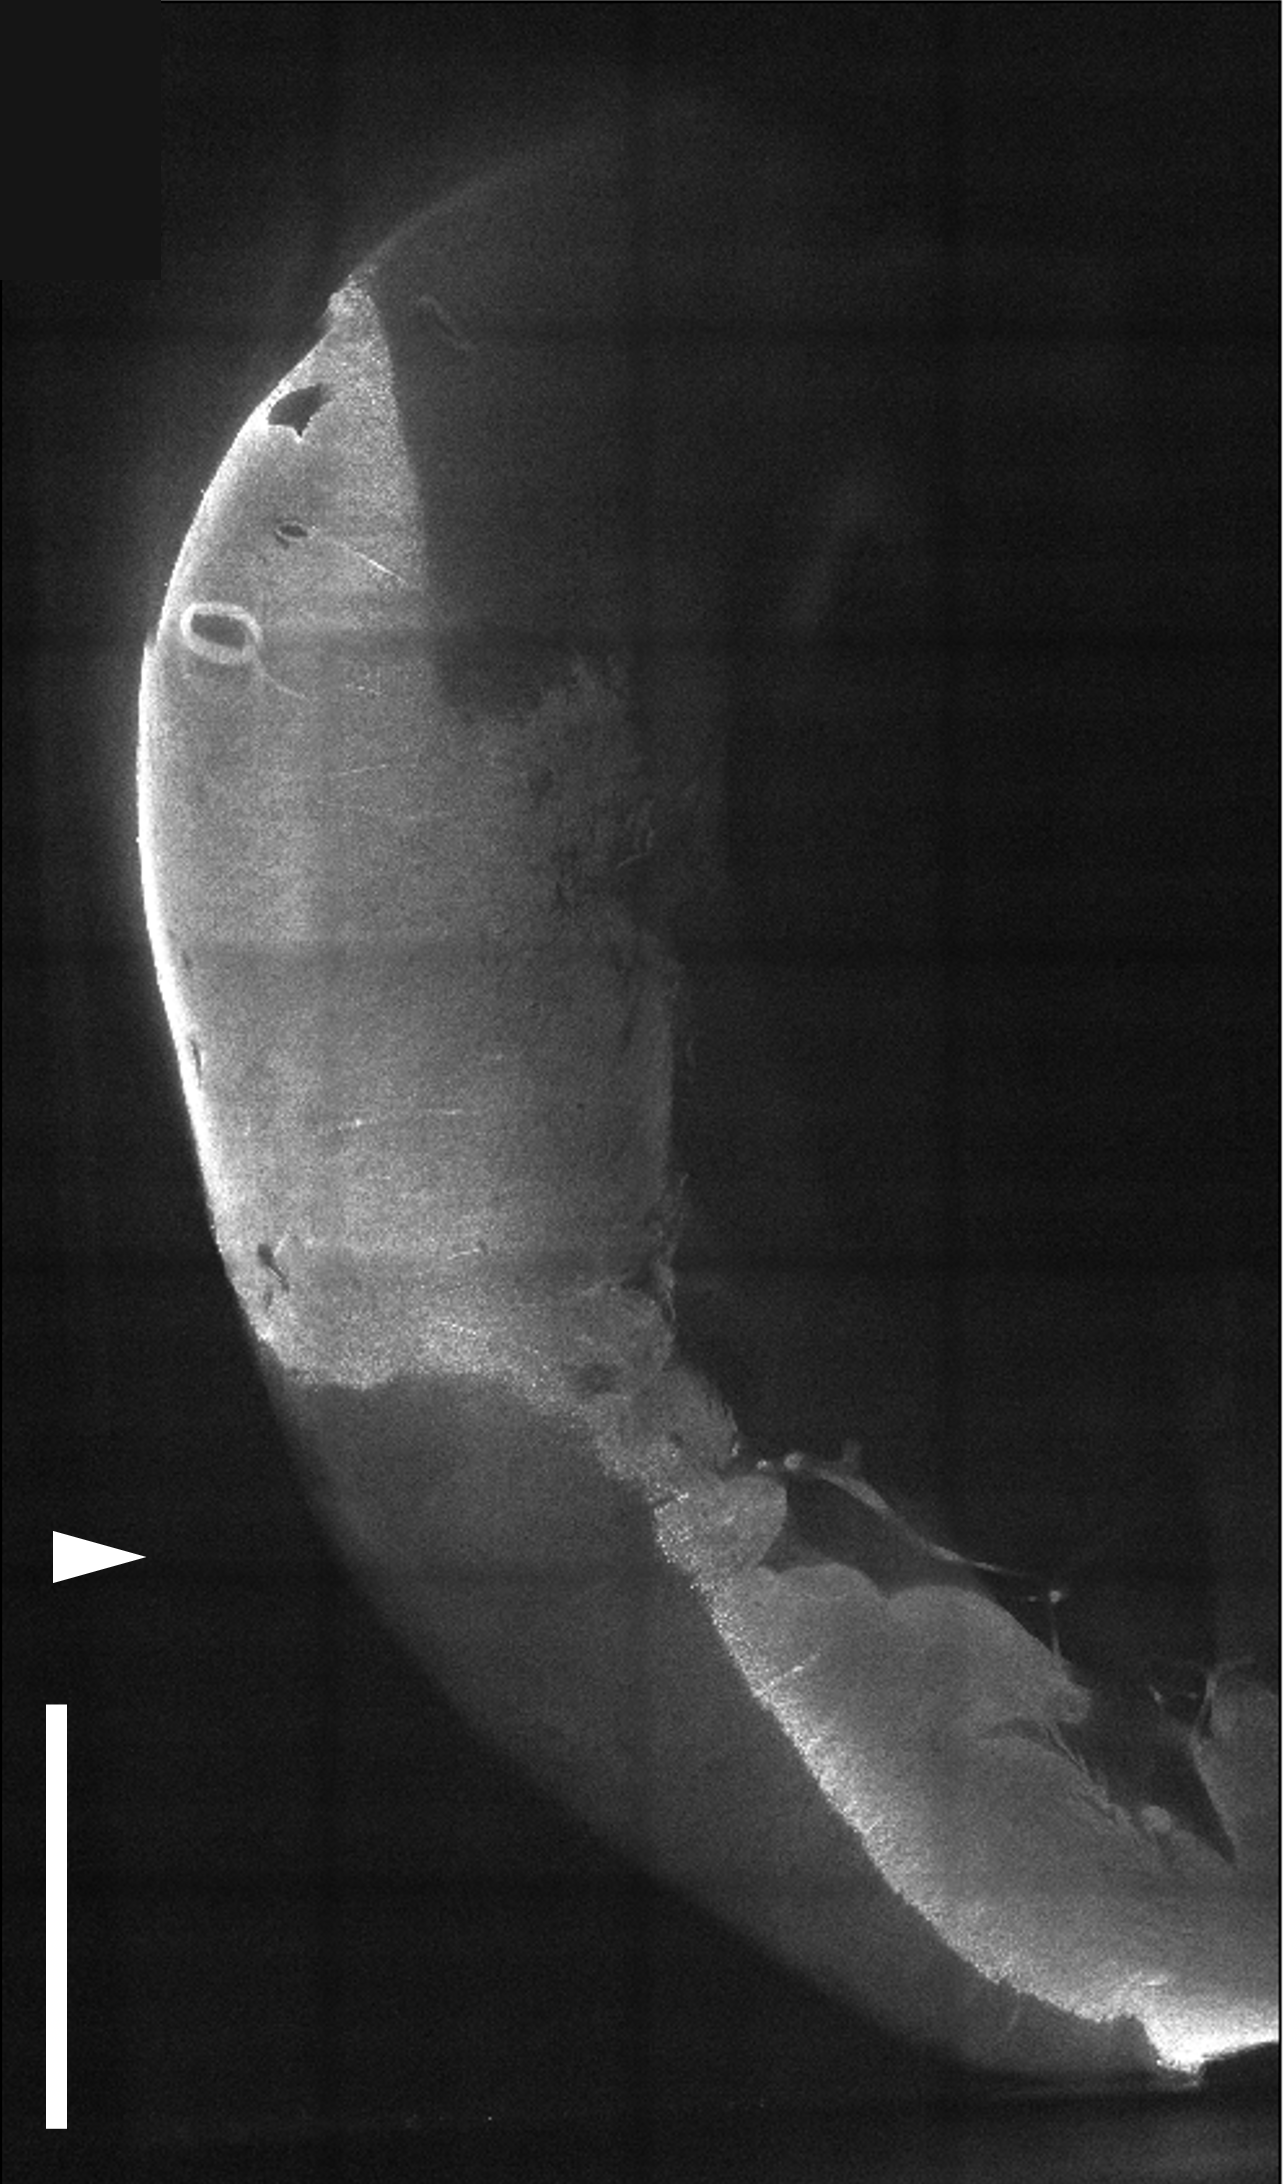
\includegraphics[width=1\linewidth]{Images/T_Sham_R_Figure_Draft_488.png}
        \caption{\textbf{488 nm Channel.} Stained using WGA/AF-488, Z = 750 microns}
    \end{subfigure}
        \medskip
    ~
    \begin{subfigure}[t]{0.48\textwidth}
        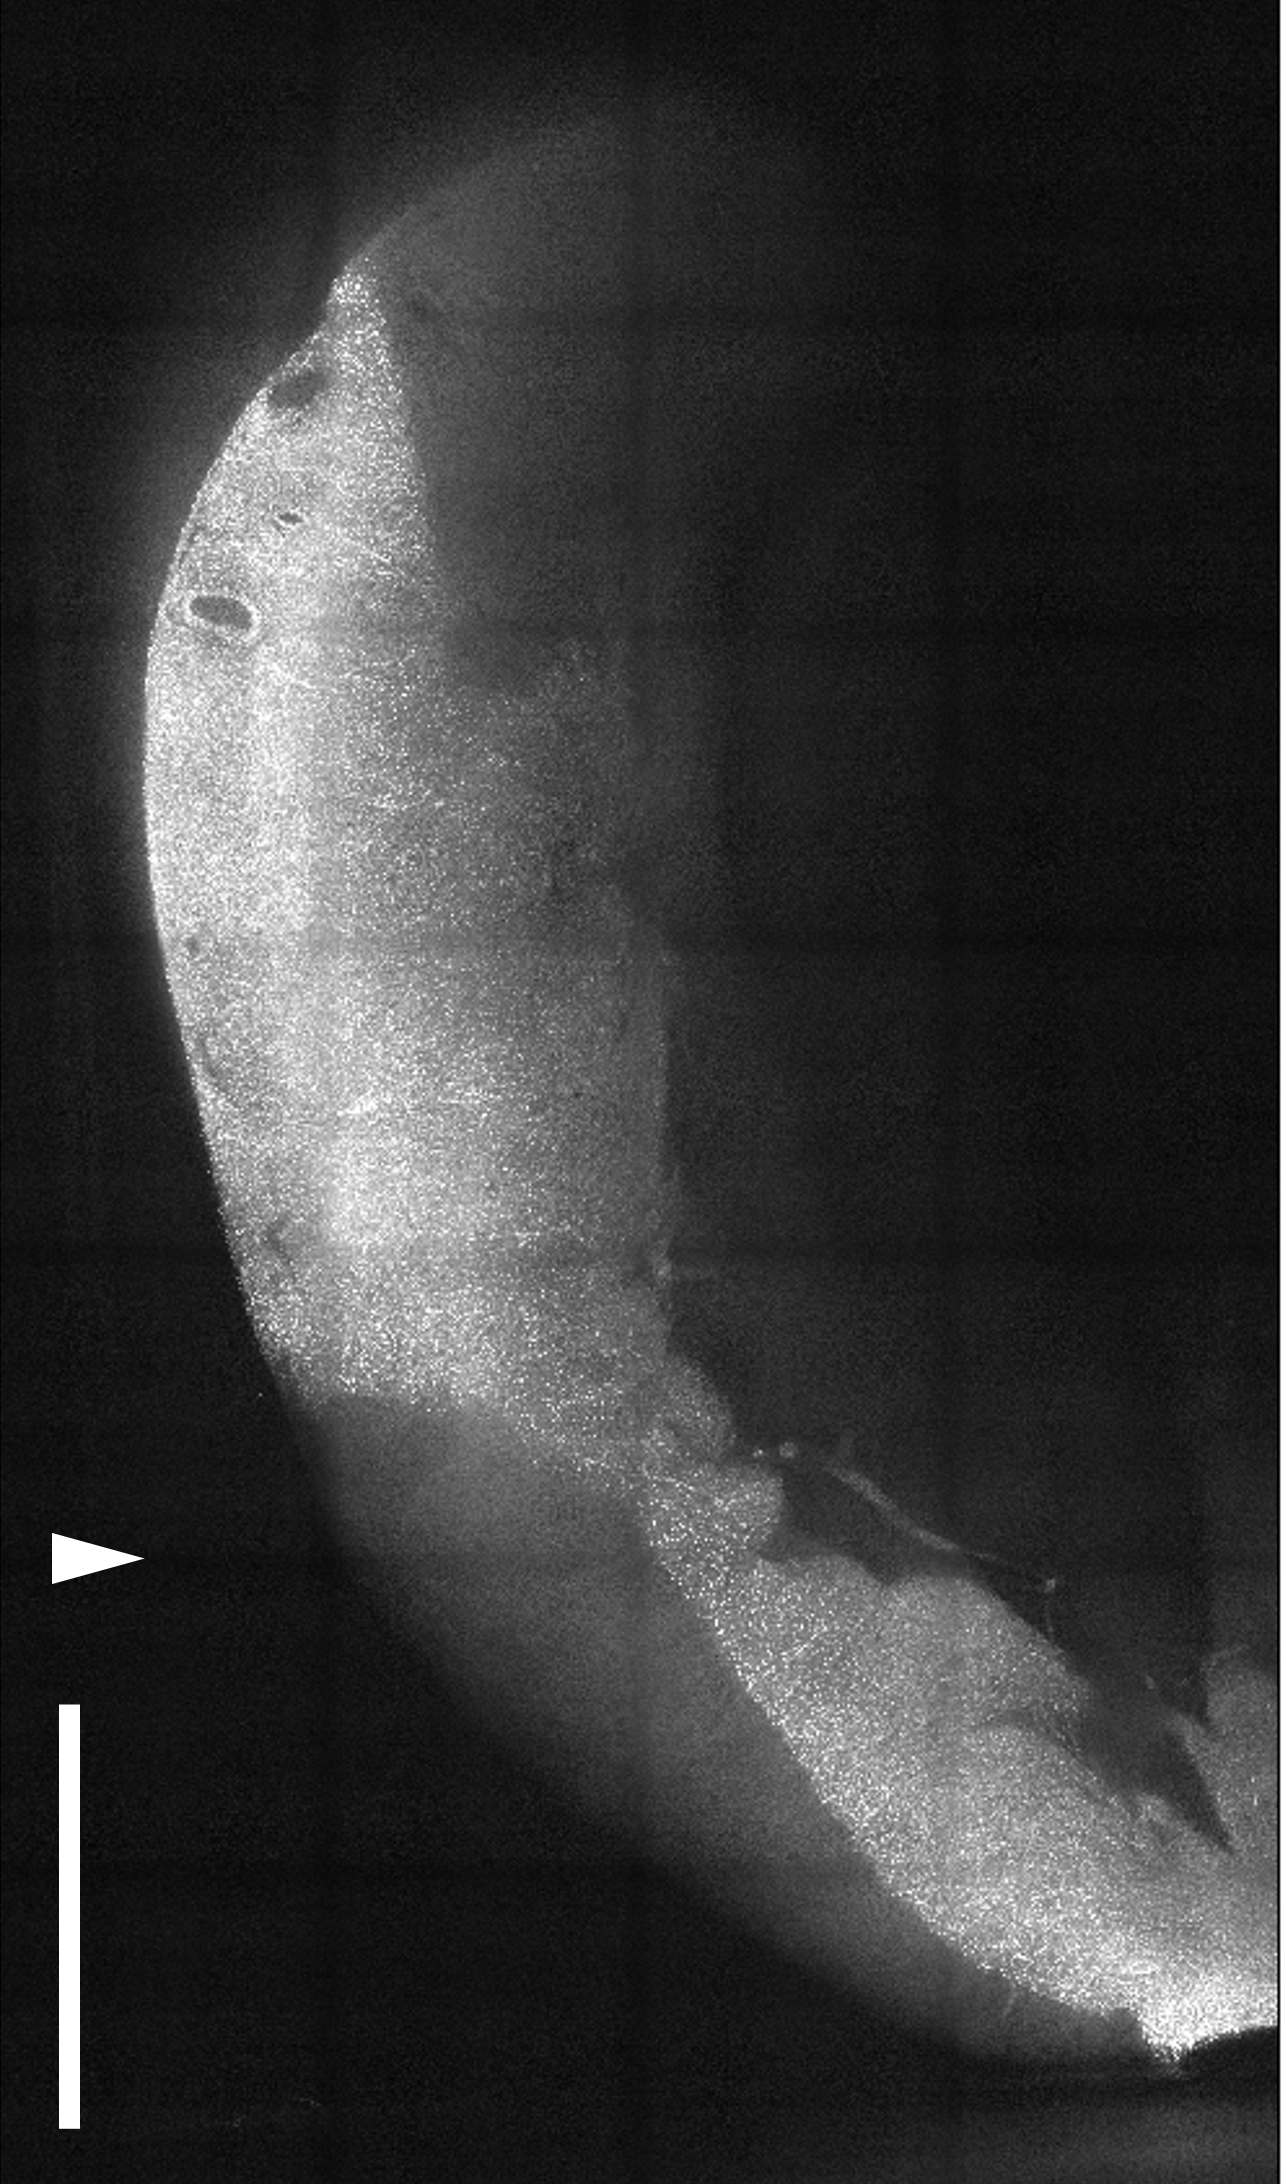
\includegraphics[width=1\linewidth]{Images/T_Sham_R_Figure_Draft_532.png}
        \caption{\textbf{532 nm Channel.} Stained using PI, Z = 750 microns}
    \end{subfigure}    
    
\caption{\textbf{Overview images of sample 38E2 T Sham R at Z = 3000 microns.} Initial layer of tissue volume imaged at Z = 0. Scale bar = 5000 microns. White triangle indicates direction of excitation incident light travel across tissue.}  
\label{fig:enter-label}
\end{figure}


\begin{figure}[H]
    \centering
        \includegraphics[width=0.75\linewidth]{Images/T_Sham_R_Figure_MIP.png}
        \caption{\textbf{MIP overlay of 488 nm (Cyan, WGA-AF/488) and 532 nm (Magenta, PI) Channels, Z = 750 to 762 microns.} Inset displays orientation of sample XY axis plane image in XZ Axis. White triangle indicates direction of excitation incident light travel across tissue. Black triangle indicated direction of emission light travel towards camera.}
        \label{fig:enter-label}
\end{figure}



\begin{figure}[H]
\includegraphics[width=1\linewidth]{Images/T_Sham_R_Figure_Draft2.png}
\caption{\textbf{Select ROIs (a-h) of MIP image of sample 38E2 T Sham R.} Z = 750-762 microns beneath initial layer. Overview of ROI locations in upper left corner, scale bar of overview = 5000 microns. Dual channel overlay (WGA/AF-488 in cyan, PI in magenta). Scale bar of ROIs (a-h) = 500 microns.}
\label{fig:enter-label}
\end{figure}

Images acquired from the light sheet positioned 3000 to 3018 microns deep into the LV section tissue volume are showcased in Figures 5.9-11. 

\begin{figure}[H]
\centering
    \begin{subfigure}[t]{0.48\textwidth}
        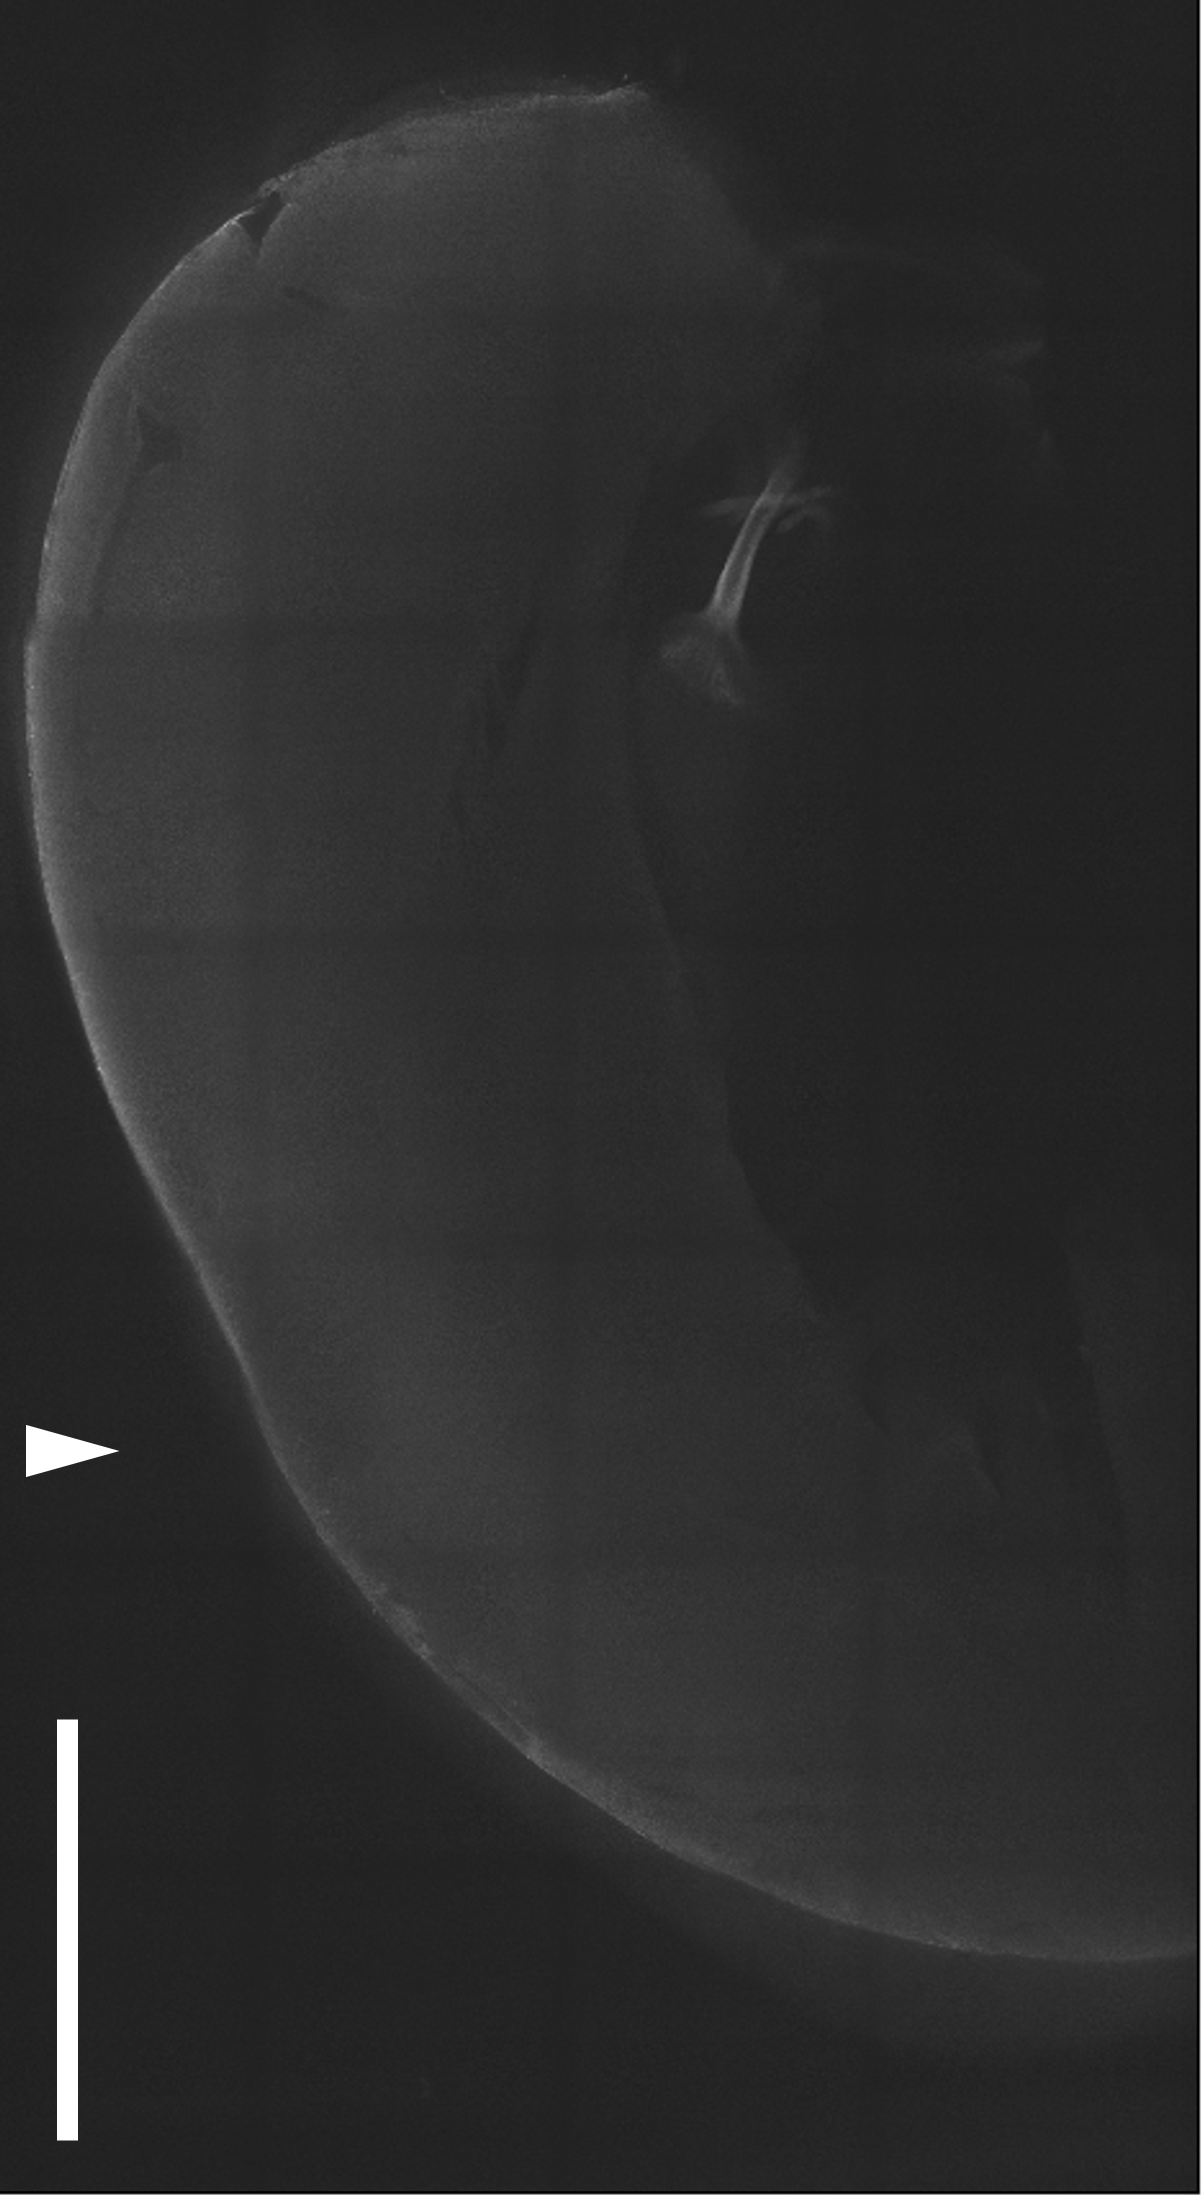
\includegraphics[width=1\linewidth]{Images/T_Sham_R_Figure_Draft_488_2.png}
        \caption{\textbf{488 nm Channel.} Stained using WGA/AF-488, Z = 750 microns}
    \end{subfigure}
        \medskip
    ~
    \begin{subfigure}[t]{0.48\textwidth}
        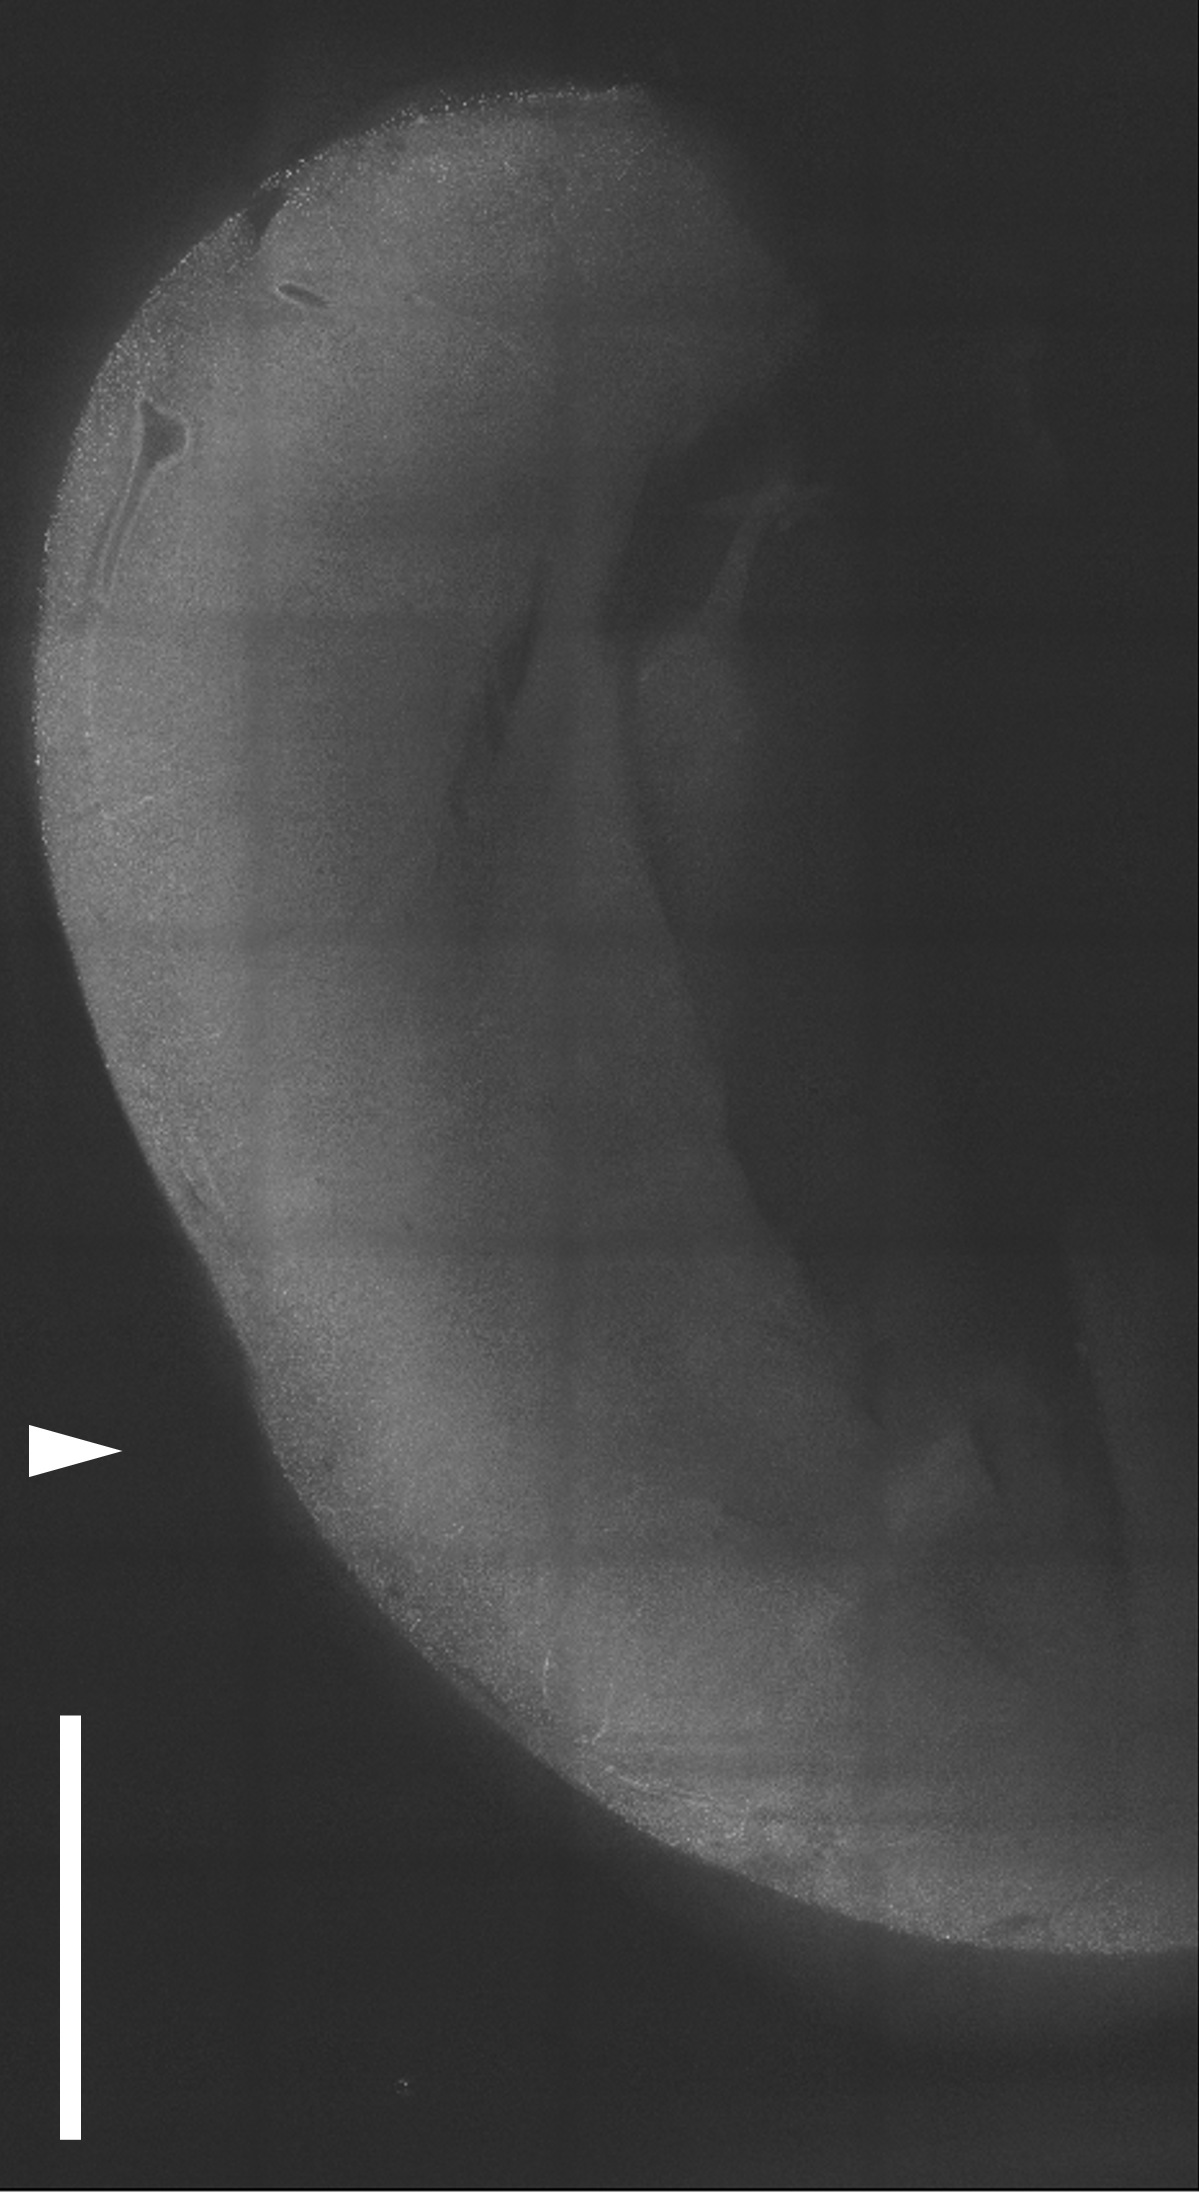
\includegraphics[width=1\linewidth]{Images/T_Sham_R_Figure_Draft_532_2.png}
        \caption{\textbf{532 nm Channel.} Stained using WGA/AF-488, Z = 750 microns}
    \end{subfigure}    
    
\caption{\textbf{Overview images of sample 38E2 T Sham R at Z = 3000 microns.} Initial layer of tissue volume imaged at Z = 0. White triangle indicates direction of excitation incident light travel across tissue.}  
\label{fig:enter-label}
\end{figure}


\begin{figure}[H]
    \centering
        \includegraphics[width=0.75\linewidth]{Images/T_Sham_R_Figure_MIP2.png}
        \caption{\textbf{MIP overlay of 488 nm (Cyan, WGA/AF-488) and 532 nm (Magenta, PI) channels, Z = 3000 to 3018 microns.} Inset displays orientation of sample XY axis plane image in XZ Axis. White triangle indicates direction of excitation incident light travel across tissue. Black triangles indicate direction of emission light travel towards camera.}
        \label{fig:enter-label}
\end{figure}
        


\begin{figure}[H]
\includegraphics[width=1\linewidth]{Images/T_Sham_R_Figure_Draft3.png}
\caption{\textbf{Select ROIs (a-h) of MIP image of sample 38E2 T Sham R at Z = 3000 microns.} Z = 3000-3018 microns beneath initial layer. Overview of ROI locations in upper left corner, scale bar of overview = 5000 microns. Dual channel overlay (WGA/AF-488 in cyan, PI in magenta). Scale bar of ROIs (a-d) = 500 microns.}
\label{fig:enter-label}
\end{figure}

As seen in all images acquired from 38E2 T Sham R, the imaging pipeline successfully acquired images of the cardiac tissue structures with the WGA-AF 488/ PI staining combination. While no attempt was made to quantitatively analyse the quality of images produced, qualitative analysis of stitched images was able to successfully identify structures native to the myocardium. The epicardium and endocardium of the tissue section are easily identifiable with blood vessels traversing the myocardium volume between them appearing with high contrast that becomes more prominent in MIP images that tracks the movement of the vessel through the tissue as it passes through the axial layers of the sample.

Comparing the image frames obtained at 750 and 3000 micron depths into the tissue volume, a noticeable degradation in fluorescent resolution is observed as the resolution capable of discerning individual cell nuclei is seen across the tissue at a depth of 750 micron (Figure 5.7(c)) but is only seen in the volume of tissue that is within approximately 2500 microns of epicardium at 3000 microns (Figure 5.9(c)). The degradation in fluorescent intensity is far more noticeable when the 488 and 532 nm channels are viewed individually. While both channels prominently illuminate the entire cross sectional area of the tissue at 750 micron depth (Figure 5.7(a-b)), at the 3000 micron depth only the 532 nm channel (Figure 5.9(b)) is able to illuminate the sample past the epicardium with sufficiently high contrast to easily discern the tissue volume from the background. The 488 nm channel at 3000 micron depth is only sufficient to discern the tissue closest to the epicardial surface of the tissue and is barely able to discern the endocardial surface on the opposite side. These findings are consistent with previous conducted spectrometer tests using CUBIC-L/RA cleared cardiac tissue (see Chapter 3, Section 2.3) which found transmission of light across these tissues to increase by roughly 20.5\% between 488 and 532 nm (wavelengths of incidence excitation light) and by roughly 37.5\% between 519 and 617 nm (respective wavelengths of fluorescent dyes emission). The increase light scattering of excitation light would explain the lower signal intensity seen in the endocardium of the sample, which was positioned away from the excitation light source. Similarly the light scattering increase of emitted fluorescent light would also explain the significant decrease in illumination at greater depths into the tissue, with the lower wavelength light emitted in the 488 nm channel degrading at a considerably faster rate compared to the 532 nm channel.

While thoracotomy adhesions to the tissue structural were minimal in this examined sample (as the thoracotomy performed in this sample was a sham procedure that saw no coronary ligations actually performed on the heart once the chest cavity was opened), some of the structural features seen in the images acquired could still serve as indicators that this invasive procedure was previously performed on this sample. This included regions containing significant concentration of WGA membrane staining at the epicardial surface of the sample, which contained minimal amounts of nuclei based on the amount of PI staining seen in these regions. Examples of these nuclei sparse regions can be seen in both images recorded of tissue structure at the 750 and 3000 micron tissue depths (Figure 5.8 (f-g) and Figure 5.9 (c-d), respectively). The persistent presence of this region regardless of changes in resolution with increase tissue depth, as well as the fact no such feature appears elsewhere in the image such as the endocardial surface, indicates that this regions is a unique characteristic of the epicardium spanning the entire three dimensional surface area of the organ present in this section. 

\subsection{Application Discussion}
\subsubsection{\textit{Thoracotomy Sham Sample Membrane and Nuclear Stain Discussion}}
The CUBIC-L/RA cleared LV section stained in the cell membranes and nuclei was examined only qualitatively in this instance as the the primary goal of the experiment at this time was to demonstrate that structural differences between percutaneous and thoracotomy induce MI models images could be observed utilizing the tissue clearing pipeline with sufficient resolution and detail to allow subsequent analysis of nuclei density, orientation, and overall cell morphology across the sample. Promising results towards this goal were obtained, as staining was shown to have successfully generated high resolution images across the cleared and stained tissue samples processed thus far. Staining specificity was also found to be maintained with nuclear stains only concentrating within cell nuclei and the WGA conjugate stain covering the cell membranes of the tissue as expected. With these results, image processing can proceed with the remaining 7 samples cleared, stained, and imaged alongside sample 38E2 T Sham R which they can be compared against. How changes in these surgical variables alter the condition and ability of the imaging pipeline to obtain high resolution images of the tissue volumes is the next question to be answered and data processing to that end is already underway as this investigation proceeds past the conclusion of this research project.


\subsubsection{\textit{Thoracotomy Sham Sample Imaging Depth Discussion}}
As discussed previously, the degradation in image resolution and contrast across the axial and lateral axes of the imaging field of view was a limitation of the lower quality of tissue clearing that is achievable with CUBIC-L/RA in comparison to CLARITY. Initial cross sectional layers of the tissue volume (which have the least amount of tissue between the light sheet and objective lens of the mesoSPIM detection pathway) provided detailed images of tissue structure and morphology that were of similar qualitative quality as what was seen with CLARITY cleared tissue slices. That similar quality however is decimated by the time the light sheet reaches the midway point through the axial tissue depth, with subsequent cross sectional layers in the back half volume of the tissue becoming barely discernable from the background signal surrounding it.  

Thankfully, there exists multiple techniques that can be applied in future imaging and data processing of LV section samples cleared and stained in a similar matter. The first of these is the re-introduction of dual-sided light sheet excitation, which will allow the excitation light to be emitted from opposite sides of the tissue, reducing the decrease in fluorescent emission die to light scattering across the tissue cross section. The left excitation are of the mesoSPIM was deactivated to increase the maximum power achievable by the right side excitation arm. Should a more powerful laser line and beam splitter be installed into the laser engine, or an altogether separate laser engine be attached to the left excitation arm, high power laser emission can be maintained in both arms to allow this feature of the mesoSPIM system to be utilized.

The second technique to mitigate signal degradation observed in this experiment is the use of the mesoSPIM system sample gantry stage to rotate the sample 180 degrees to allow the back half of the tissue volume to face the objective lens. Imaging of the sample in this orientation will illuminate the back half of the sample with the same intensity and resolution as the front half of the sample would have achieved. The two image sets could then be recombined digitally with the high resolution images of the front and back halves of the volume now contained in a single stack for subsequent post-processing. Obtaining this type of data set will require the removal of the agarose bed used to support tissue slices narrower than the inner cuvette used in imaging, as the high concentration agarose gelatin will obstruct the detection path's view of the sample if rotated 180 degrees. This will open the sample up to freely move within the inner cuvette as the mount is rotated and shifted in the course of multi-tile imaging, making any attempt to combine the image stacks taken into one contiguous image stack impossible. To support the sample and keep it stationary, it would therefore be necessary to use inner cuvettes with customized dimensions to properly fit these thinner samples without the need for additional agarose bed support. 

\subsubsection{\textit{LV Section Data Processing Discussion}}

One aspect of imaging LV sections cleared and stained using the imaging pipeline and the staining protocol established in this chapter section that must be highlighted as a potential issue in future attempts is the considerable amount of time, storage, and processing power that is required from PC systems utilized in the post processing steps of the imaging pipeline applied here. The size of data sets and files created for this investigation were, by far, the largest created and processed through the imaging pipeline. For the 8 LV section samples imaged, to record the entire tissue volume in just one channel, an average of 42 tiles was required to cover the entire sample with 10\% overlay between each tile's FOVs. This averaged to a total data set size of 2.16 TBs per sample per channel imaged. In total, 34.5 TB of raw data were recorded, all of which would need to undergo extensive post processing utilizing IMARIS and ImageJ software. Limited access to the IMARIS software licensed PC in combination with the limited speeds at which data can transfer to/from the mesoSPIM PC NAS (see Chapter 2, Section 4.4) means the processing of this massive data collection will require months to complete. As a result, only 1 out of the 8 samples (38E2 T Sham R) could be fully processed in time to be examined and presented here. 

Steps should be taken in future endeavours utilizing this imaging pipeline with such large volumes of data to ensure a more smooth and efficient post processing system is in place to mitigate these challenges. This is especially true should dual sided excitation and 180 degree cuvette rotated imaging be attempted as previous described. The implementation of these methods will result in raw data sets for a single sample being quadrupled in size from the very start of post-processing as the entire volume of the tissue will undergo imaging 8 times (2 channels x 2 excitation directions x 2 angles of orientation = 8 unique image stacks). Further details regarding recommendations towards resolving these processing issues along with other improvements that can be made to the overall imaging pipeline can be found in Chapter 7, Section 1.2.



\section{Rabbit LV Spheroid Injections for Regenerative Medicine}
This project was conducted in collaboration with Ms. Sasha Forbes at the School of Cardiovascular and Metabolic Health, College of Medical, Veterinary, and Life Sciences, University of Glasgow. Steps 1-5 in the tissue processing pipeline (Figure 1.1) were conducted by Ms. Forbes with subsequent imaging and data post processing completed by Ms. Sasha Forbes, Dr. Eline Huethorst, Dr. Sharika Mohanan, Mr. Ahmed Elnageh, and myself using the mesoSPIM microscope in combination with Fiji ImageJ, BigStitcher, and IMARIS softwares for data processing \cite{schindelin_fiji_2012,noauthor_imaris_2024, horl_bigstitcher_2019}. 

\subsection{Experimental Concepts}
\subsubsection{\textit{Background}}
One of the most prominent goals in the field of regenerative medicine is to find methods by which healthy cardiac activity post-MI can be restored through means of medical intervention. Prior research in the field explored sub-epicardial engrafting of engineered heart tissues a means by which this treatment could be introduced into the damaged organ. This research built upon research exploring the intra-myocardial injection of cells and proved that this methods of implantation has potential to restore heart activity and prevent future heart failure \cite{gerbin_winding_2015, huethorst_evidence_2025}. 

It is believed that the use of spheroids, containing stem or cardiac cells, instead of engineered tissue could prove to be a more effective means of integrating new, healthy tissue into the existing myocardial tissue structure. It is hypothesized that higher degrees of integration into the surrounding cardiomyocytes aids in the ability of the spheroid cells to synchronize contractions with the organ. This can reduce the potential of the engraftment to generate ventricular arrhythmias because of poor electrical coupling, which was seen in previous research utilizing engineered heart tissue engraftments \cite{gerbin_winding_2015}.

The objective of this project is to gain a better understanding of the tissue structure that surrounds spheroids injected via syringe beneath the epicardial surface of host hearts. The ultimate goal of these observations is to determine the impact, if any, the spheroids may have in the electrical activity of healthy and infarct hearts stemming from these physical interactions.  This will be achieved by combining the structural information obtained via cleared tissue imaging with existing functional data acquired from theses host hearts beforehand. The retention rate and dispersion of spheroids once engrafted into the sub-epicardium are additional aspects of the procedure aimed to be better understood through examination of the tissue and remaining spheroid grafts located at the injection site. Should restoration of healthy cardiac activity be achieved by this methods of spheroid injection, it is hoped that the concept could serve as a basis in the distant future by which regeneration of healthy, normal cardiac activity post-MI can be regularly achieved.  



\subsubsection{\textit{Methodologies}}
\paragraph{Spheroid Sample Preparation, Acquisition}
For this project, 4 leporine hearts were excised and placed onto Langendorff perfusion set up (see chapter 2, section 1). Each heart than has spheroids injected via syringe several microns beneath the surface of the LV epicardium. One sample is injected with spheroids containing Human induced Pluripotent Stem Cells (HiPSC; Celo.Cardiomyocytes, Celogics) while the other 3 samples were injected with rat myofibroblast cells (H9C2 Cell Line; American Type Culture Collection, CRL-1446). While still perfusing, hearts undergo real time functional analysis using calcium dyes and electrodes, respectively, to record a pseudo-Echocardiogram (pECG) from the excised hearts \cite{huethorst_evidence_2025}. 

After functional analysis is completed, the left ventricle exterior wall of hearts with strong spheroid signals are excised and cut into segments containing roughly 1 \(cm^2\) of the Epicardium surface area each. Sections are cut to have the site of spheroid injections located at or near the midpoint of each tissue section. A suture is tied to the surface of the epicardium several millimetres above the injection site to aid in spheroid location post-clearing. From here, the pipeline protocol for CUBIC-L/RA tissue clearing of left ventricle sections is performed as detailed in Chapter 3.

Prior to immersion in CUBIC-RA, CUBIC-L treated tissue sections were stained using a combination of a WGA conjugated membrane dye (WGA/AF-555 or WGA/AF-647) and the nucleic acid dye SYTOX Green. Staining protocol followed was identical to the protocol described in the previous chapter section, described step by step in Table 5.2. Stains used on each of the 4 samples created are listed in the following table allong with naming conventions for each sample:


\begin{table}[H]
    \centering
    \begin{tabular}{|c|c|c|}
    \hline
         \textbf{Sample Name} & \textbf{Cell Membrane Stain} & \textbf{Cell Nuclei Stain} \\
         \empty & \textit{WGA Conjugate Dyes} & \textit{Nucleic Acid Dyes}\\
         \hline
        HiPSC 4.2 & AF-647 & SYTOX Green\\
        H9C2 5.1 & AF-647 & SYTOX Green\\
        H9C2 5.2 & AF-647 & SYTOX Green\\
        H9C2 5.3 & AF-555 & SYTOX Green\\
    \hline
    \end{tabular}
    
    \caption{\textbf{Spheroid injected sample tissue staining and naming conventions.}}
    \label{tab:placeholder}
\end{table}



\subsection{Experimental Results}

Imaging was performed on all 4 LV sections in the 488 nm channel along with the 532 nm channel (for sample H9C2 5.3) or 647 nm channels (for samples HiPSC-4.2, H9C2-5.1, and H9C2-5.2). Spheroid injection sites were searched for using the attached suture knot as an identifiable landmark to use as a starting point for the search. The syringe injection would leave behind a straight channel through the tissue of the epicardium and end several microns beneath the epicardial surface. Once the channel is located, the light sheet would be shifted across the length of the channel to confirm the channel is not mistaken for a blood vessel in the tissue, which has similar appearance to the syringe channel in acquired images. To distinguish syringe channels from vessels, the walls of the structure are examined to see if they resemble the jagged, coarse patterns expected to be created artificially in the tissue by the syringe needle. 

Once confirmed, the channel is then examined for the presence of spheroids, which emit strong fluorescent signals in both channels compared to the surrounding weaker signal emitted by the myocardial tissue. Once the spheroids are located inside or near the syringe channel, the location of the site in relation to the suture knot is recorded to allow for future imaging sessions of these sample to quickly relocate these ROIs. Image recording and processing of the syringe channel structures proceeds as laid out in the tissue imaging pipeline. Image stacks recorded were set to begin approximately 30-36 micron (10-12 steps in z-axis) before the appearance of the syringe channel. The image stack would extend through the layers of tissue containing the spheroids and is set to end recording roughly 36 microns past the final frames in which the spheroids and syringe channel are visible. 

Maximum intensity projections (MIPs) of multiple frames acquired during imaging were created for each sample using Fiji ImageJ software. These projections overlay 5 frames (15 microns in z-axis) in the recorded tissue volume where spheroids are most visible in the FOV. In samples where spheroids spanned across more than one image tile, BigStitcher was used to stitch adjacent MIPs together into single frames covering the complete ROI. Once acquired, a close up ROI is selected (roughly 0.8-1.0 $mm^2$ in size) and the image of this area is viewed in each channel individually and combined to qualitatively compare the quality of fluorescent stain emissions on the spheroids in the tissue.

\subsubsection{\textit{Human induced Pluripotent Stem Cell Spheroid Injection Sample Results}}


\begin{figure}[H]
\centering
\includegraphics[width=1\linewidth]{Images/SpheroidSample4_2.png}
\caption{\textbf{Spheroids in sample HiPSC-4.1.} Left Column: 647 nm channel MIP, middle column: 488 nm channel, right column: Composite dual channel MIP. ROI zoom in on spheroid injection highlighted in yellow in full image, shown in bottom row of respective channel. White triangle indicates direction of excitation incident light travel across tissue. Scale bars = 500 microns.}
\label{spheroids4.2}
\end{figure}

In sample HiPSC-4.2, it was seen that the HiPSCs were successfully stained by both the WGA/AF-647 and the SYTOX Green stains as seen in the individual channel images in Figure 5.13. The strongest signal intensity and image resolution was seen in the region of the syringe injection cavity closest to the edge of the epicardium where the mesoSPIM light-sheet first enters the tissue volume.

\subsubsection{\textit{WGA/AF-647, SYOTX Green Staining, H9C2 Cell Line Spheroid Injection Sample Results}}

\begin{figure}[H]
\centering
\includegraphics[width=1\linewidth]{Images/SpheroidSample5_1.png}
\caption{\textbf{Spheroids in sample H9C2-5.1.}  Left column: 647 nm channel MIP, middle column: 488 nm channel, right column: composite dual channel MIP. ROI zoom in on spheroid injection highlighted in yellow in full image, shown in bottom row of respective channel. White triangle indicates direction of excitation incident light travel across tissue.  Scale bars = 500 microns.}
\label{fig:enter-label}
\end{figure}
\medskip

\begin{figure}[H]
\centering
\includegraphics[width=1\linewidth]{Images/SpheroidSample5_2.png}
\caption{\textbf{MIP images of spheroids in sample H9C2-5.2.} Left column: 647 nm channel MIP, middle column: 488 nm channel, right column: Composite dual channel MIP. ROI zoom in on spheroid injection highlighted in yellow in full image, shown in bottom row of respective channel. White triangle indicates direction of excitation incident light travel across tissue. Scale bars = 500 microns.}
\label{fig:enter-label}
\end{figure}
\medskip

For samples H9C2 5.1 and 5.2, the syringe channel was found to traverse the tissue volume for a span longer than the existing camera FOV. For these recording, two image tiles were captured following the established mesoSPIM image tiling protocol (see chapter 2, section 3.2) and stitched together in post-processing to allow examination of the channel in its entirety. At most, spheroid dense regions located in these samples required 2 image tiles in a [2x1] image matrix to capture the injection region in full.

\subsubsection{\textit{WGA/AF-555 Staining, SYTOX Green H9C2 Cell Line Spheroid Injection Sample Results}}

\begin{figure}[H]
\centering
\includegraphics[width=0.9\linewidth]{Images/SpheroidSample5_3.png}
\caption{\textbf{Spheroids in sample H9C2 5.3.} Top row: 532 nm channel MIP, middle row: 488 nm channel MIP, bottom row: Composite dual channel MIP. ROI zoom in on spheroid injection highlighted in yellow in full image, shown in bottom row of respective channel. White triangle indicates direction of excitation incident light travel across tissue. Scale bars = 500 microns.}
\label{fig:enter-label}
\end{figure}
\medskip

Sample H9C2-5.3 was seen to have the poorest visibility out of all 4 spheroid samples imaged and processed using the imaging pipeline. This reduced spheroid visibility was likely a result of two factors that inhibited the ability of the mesoSPIM to view the structures with the same fidelity as previously seen. 

The first factor contributing to the reduced resolution and poorer contrast seen in images acquired from sample H9C2-5.3 is the use of the 532 nm laser line in combination with WGA/AF-555, which was unique to this sample. Unlike the 647 nm channel, which has light transmittance over 95\% in CUBIC-L/RA cleared tissues (see chapter 3, section 3.2) and can illuminate the WGA/AF-647 with its highest possible relative intensity, the 532 nm channel is only capable of light transmittance in CUBIC-L/RA cleared tissues of approximately 60\% and whose fluorophore used (WGA/AF-555) are not emitting at full intensity due to the 532 nm laser line having a wavelength 23 nm shorter than what is required to have WGA/AF-555 emit light at its highest possible intensity. The factors combined reduces the overall resolution and contrast obtained when imaging the membranes of the cells in the myocardium. 	 

The second factor is that the spheroids visible in the sample appear to be located in a region farther from the surface of the epicardium compared to the other 3 samples imaged. The deeper placement of these spheroids means the spheroids are unable to take full advantage of the high resolution that is achievable in these initial layers of tissue to discern the individual spheroids and the syringe channel they should occupy. As seen in the ROI zoomed in view of the spheroids in Figure 5.16, several blood vessels were located near the spheroids that were visible in the sample, suggesting the possibility that a number of the injected spheroids may have entered these vessels deeper in the tissue volume, obscuring them from view as densely packed and brightly illuminating endothelial cells making up the vessel walls obscure spheroids from view. Supporting this theory, further visual analysis of the tissue volume was performed on tissue layers beneath the injection site region. Additional vessel structures were found to exist beneath the injection cavity and what appeared to be spheroids lodged into the largest of these vessels were observed as shown in Figure 5.17.

\begin{figure}[H]
\centering
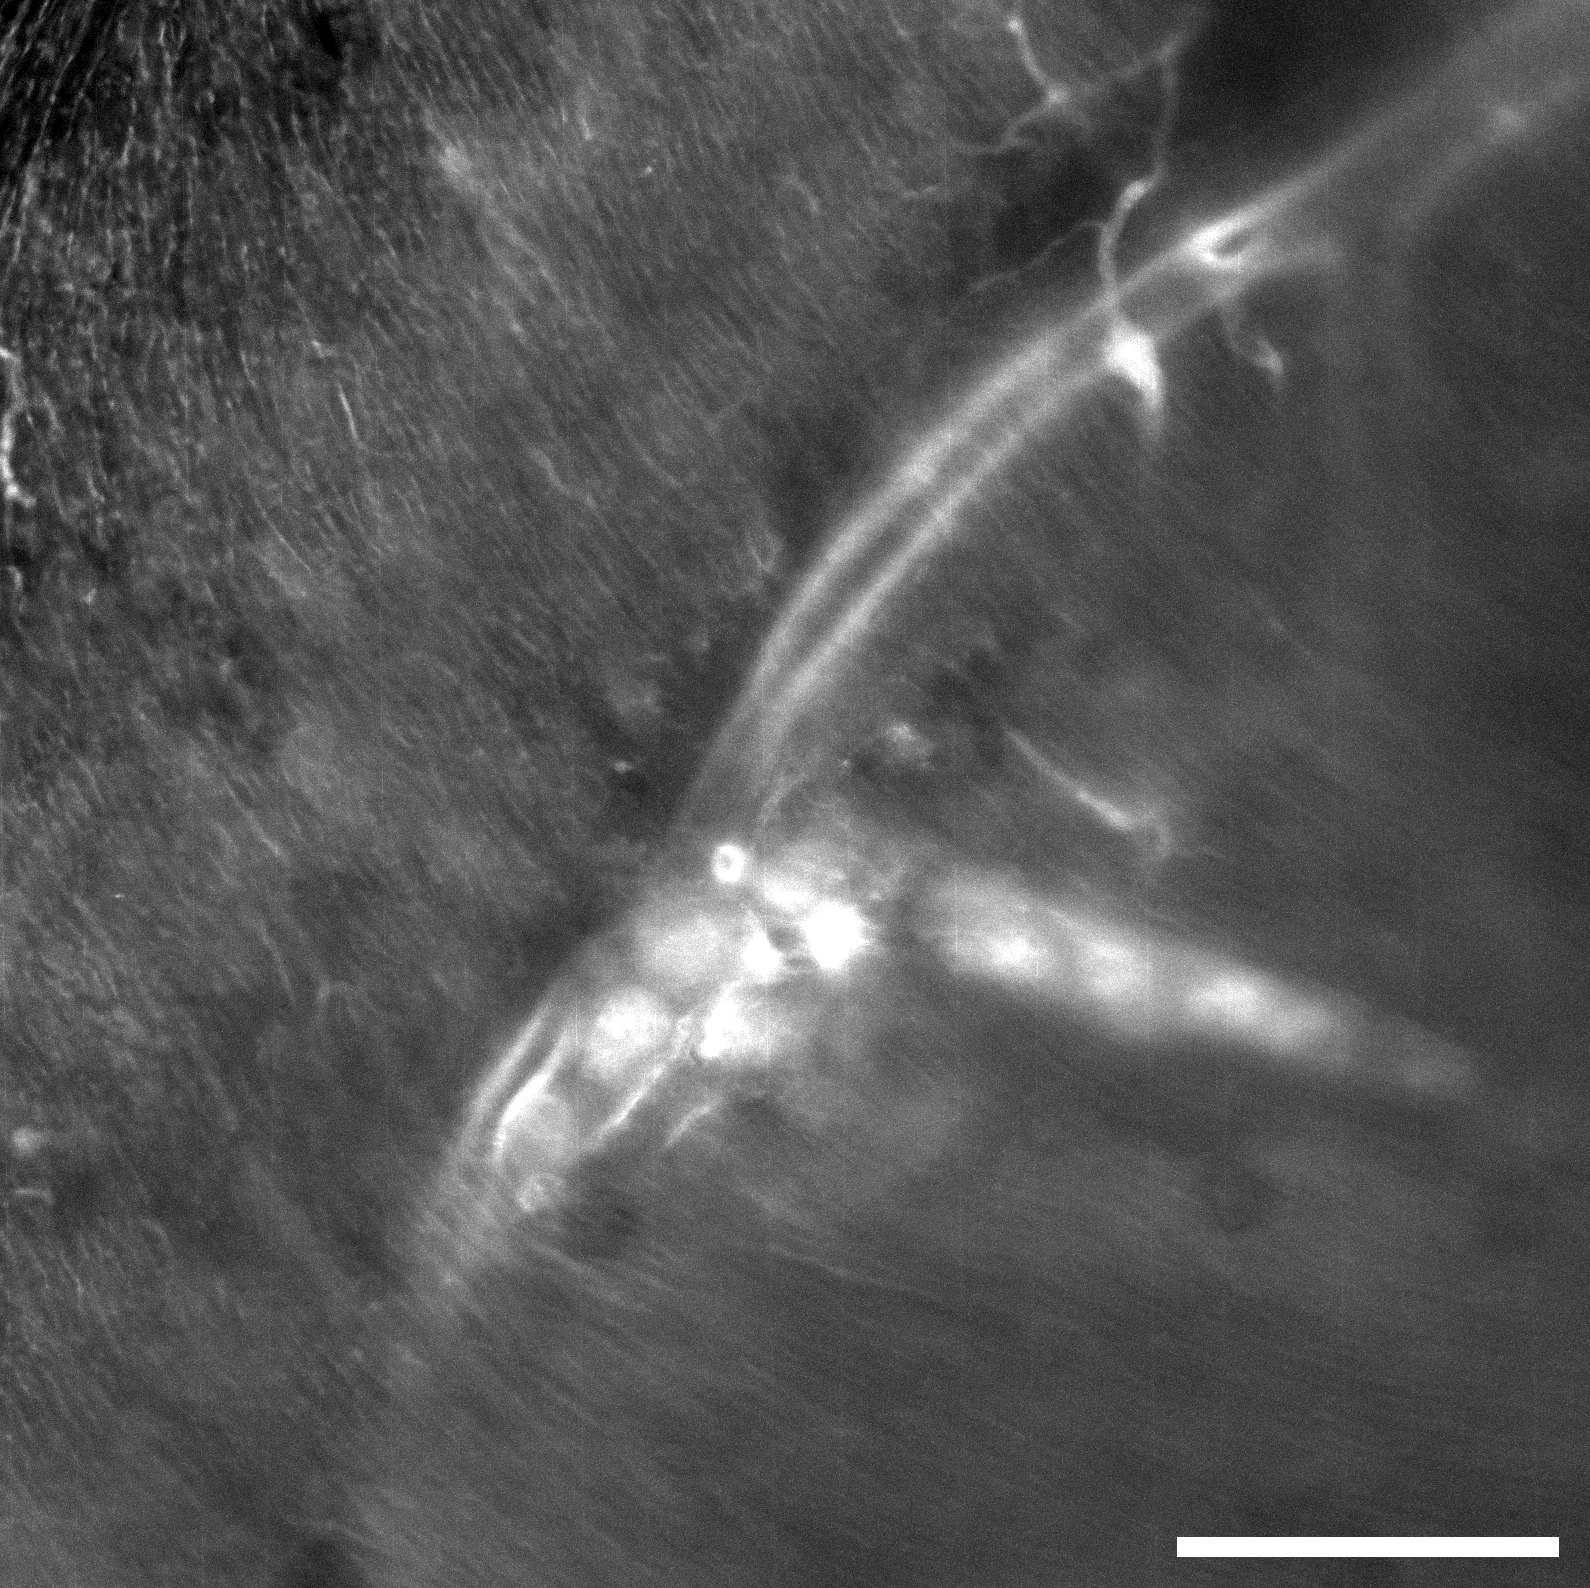
\includegraphics[width=0.5\linewidth]{Images/Spheroids_In_Vessel.png}
\caption{\textbf{Possible spheroid lodgement into coronary blood vessels in sample H9C2-5.3.} Only MIP image of channel 532 (WGA/AF-555 stain) is shown as channel 488 (SYTOX Green) of too poor contrast for proper channel overlay. Scale bars = 500 microns.}
\label{fig:enter-label}
\end{figure}
\medskip

\subsection{Application Discussion}
\subsubsection{\textit{Challenges In Mounting, Imaging Discussion}}

Unlike previous experiments in which the sample volumes were imaged in their entirety, the tissue samples injected with spheroids were recorded only in those regions where spheroids were visually observed by the microscope user in the course of looking through the tissue volume using the mesoSPIM software live camera feed. This proved to be a highly time consuming and labour intensive process compared to prior imaging protocols as the tissue would often times need to be removed from the sample gantry and the inner cuvette mount so that it can be carefully reoriented to allow the spheroid region to be as close to the light sheet emission source as possible for optimal resolution and florescent contrast in the CUBIC-L/RA cleared tissue. Performing this reorientation was frustratingly tedious to perform as the process required manually moving the tissue by hand, which is now soaked in the lubricious CUBIC-RA solution. Gentle handling of the sample would see it slip out of the grasp of any precision forceps used, while larger and broader forceps ran the risk of damaging the tissue in the process of handling. Thus slow and careful sample handling using paintbrushes and pipette tips was the only means by which the process could be properly completed. While the process was successfully completed in all samples that required it, it is still believed that eliminating the need for adjustment is the most ideal scenario for any future spheroid imaging attempts.

It was discovered after imaging the second of the four samples in the experimental sample series that the optimal orientation followed the trend of having the suture knot, which was consistently left by the spheroid injector on the epicardium a few millimetres away from the spheroid injection site, positioned towards the upper left corner of the cuvette with the epicardial face of the tissue facing the objective lens of the detection path. In this orientation, there is the least amount of tissue volumes between the injection site, the excitation light entering the cuvette, and the objective lens of the detection path. This reduces the amount of light scattering that occurs as light traverses into and out of CUBIC cleared tissue, improving the resolution of acquired images of the syringe channel and spheroids. Due to the camera being installed upside-down in the mesoSPIM detection pathway, this selected orientation positions the suture in the lower right corner of the acquired image FOV (as seen in the lower right corner of stitched images in Figure 5.15). 

This suture placement was set as the standard in the remaining 2 samples imaged, which resulted in no further adjustment of the sample position being required. A diagram and photo of this orientation in the cuvette with respect to the mesoSPIM excitation and detection path is shown below:

\begin{figure}[H]
\centering
    \begin{subfigure}[t]{0.75\textwidth}
    \centering
        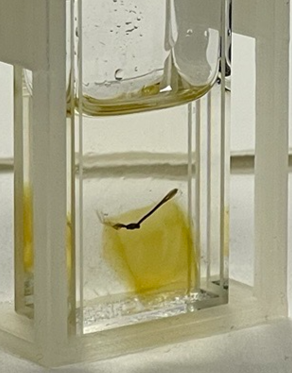
\includegraphics[width=0.5\linewidth]{Images/Spheroid Orientation.png}
        \caption{\textbf{Image of properly orientated spheroid sample in mounted inner cuvette.} Excitation light enters inner cuvette from narrow side on the left.}
        \medskip
    \end{subfigure}
            
    \begin{subfigure}[t]{0.75\textwidth}
        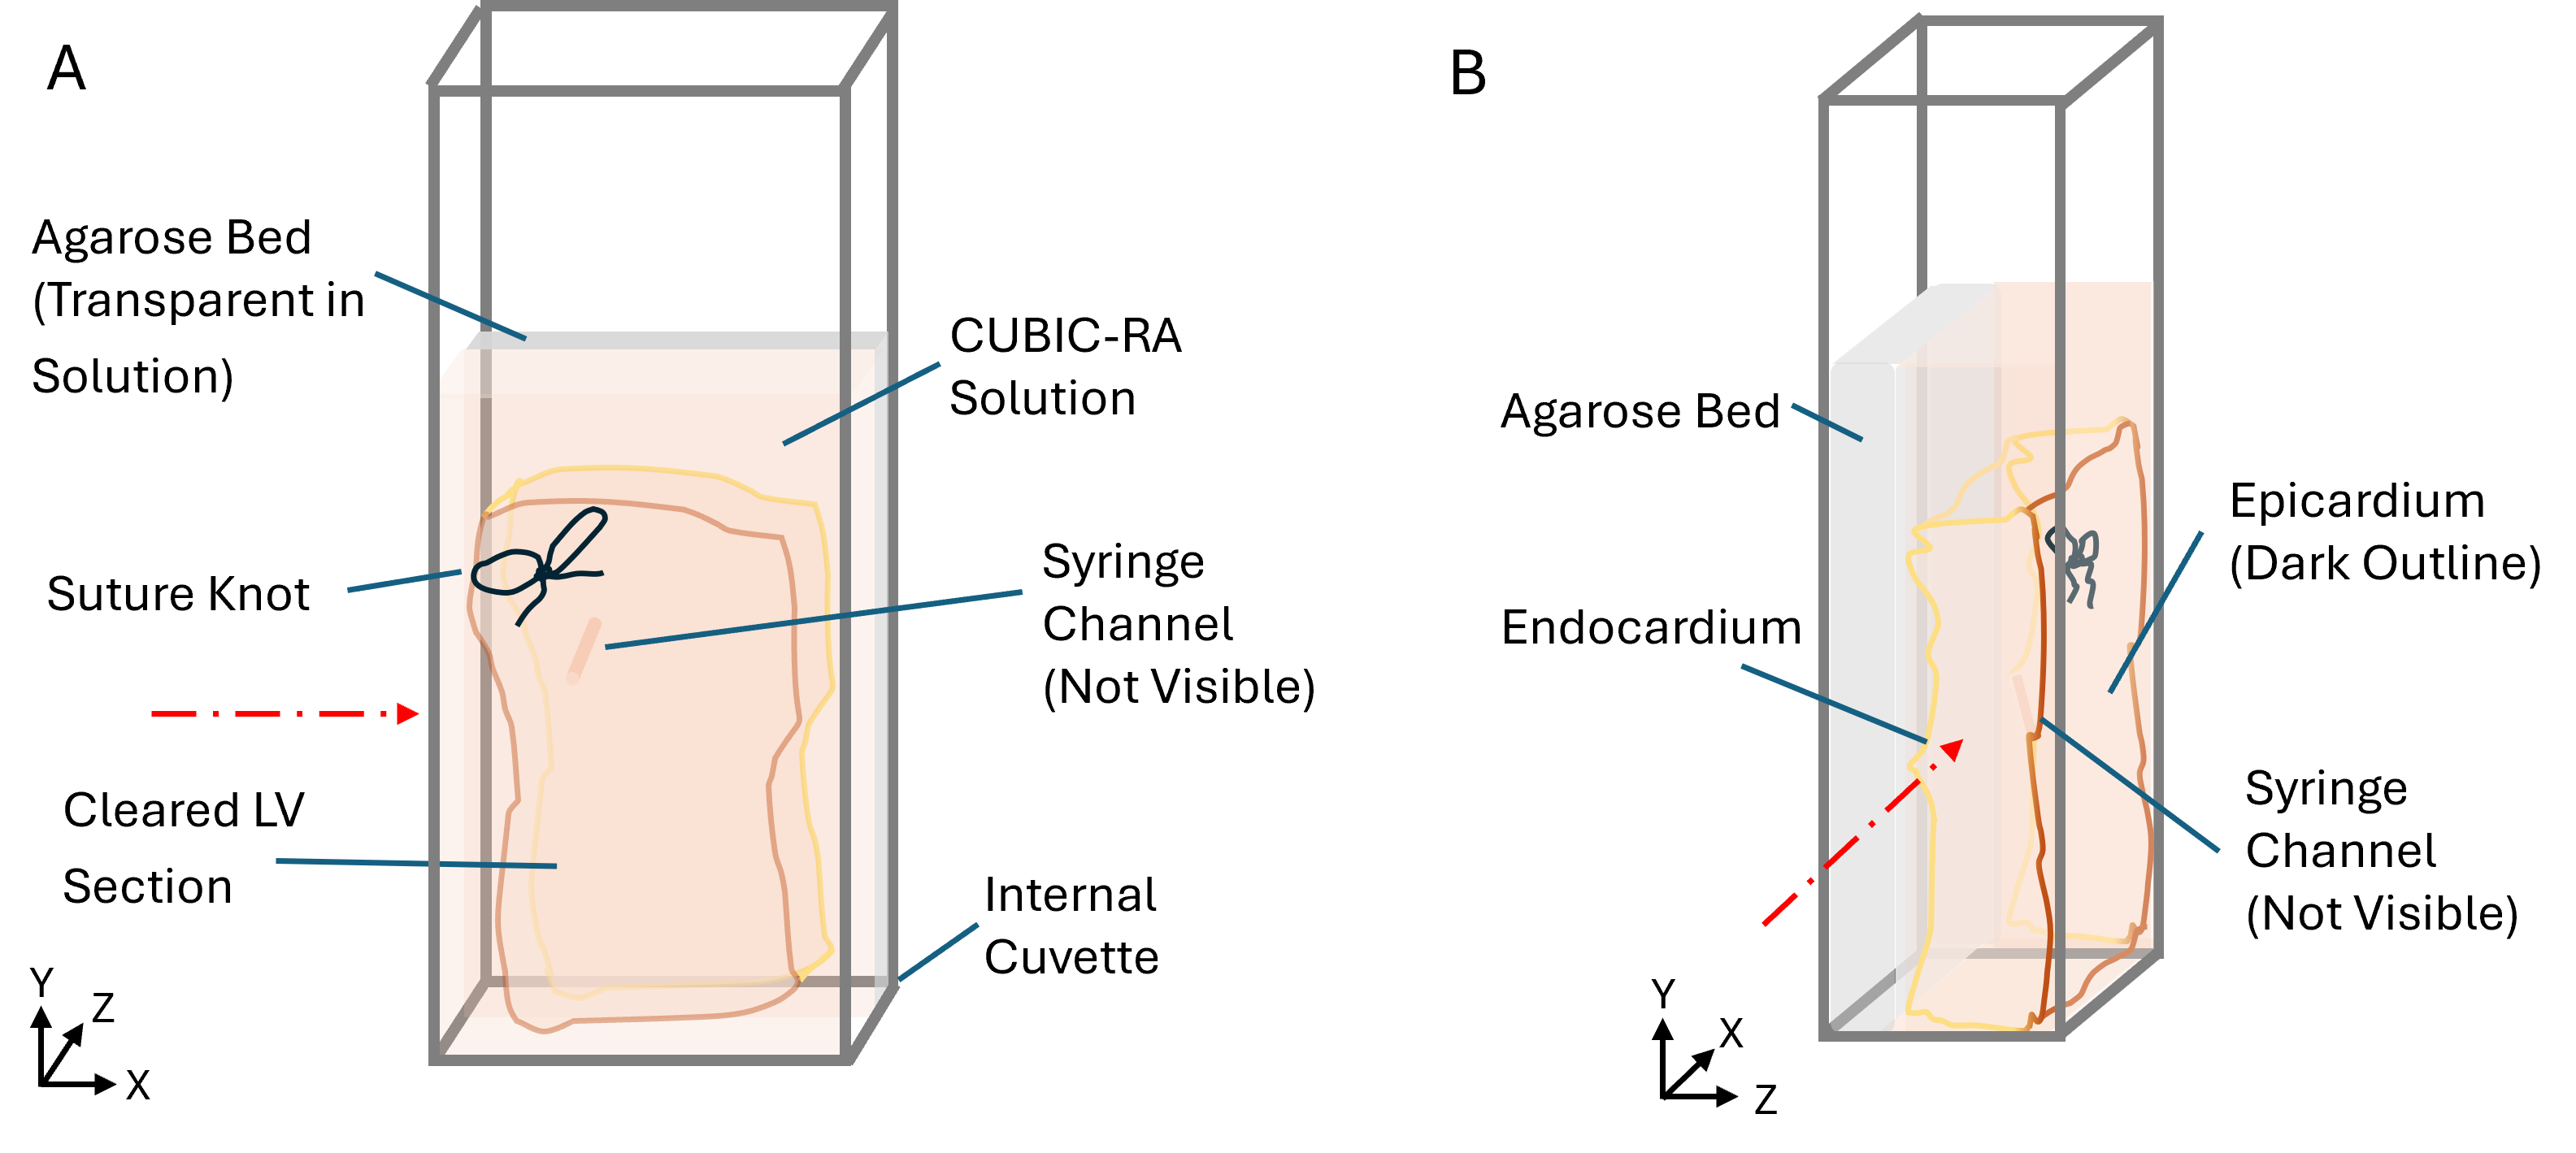
\includegraphics[width=1\linewidth]{Figures/Spheroid OrientationDiagrams.png}
        \caption{\textbf{Diagram of properly orientated sample inside cuvette} Inset A: frontal view of cuvette. Inset B: side view of cuvette. Red dashed arrow indicated direction of excitation light into cuvette during imaging (on XY-plane). Diagrams not to scale.}
        \medskip
    \end{subfigure}    
    
\caption{\textbf{Spheroid LV tissue sample orientation in inner cuvette for optimal imaging of injection site.}} 
\label{fig:enter-label}
\end{figure}

While the placement of a suture in the epicardium proved vital to the proper placement of the tissue in the inner cuvette for optimal spheroid imaging, the presence of the uncleared suture fibres in the sample proved to be problematic. Samples with sutures in place would often times have stray fibres from the suture be present on the surfaces of the tissue closest to the main suture body, these fibres would then obscure views of tissue behind the fibres in the tissue volume, blurring the view. An example of these suture fibres observed in the sample and the aberrations they induce in imaging planes deeper into the tissue sample is shown below:

\begin{figure}[H]
\centering
\includegraphics[width=0.75\linewidth]{Images/Fibre_Figure.png}
\caption{\textbf{Suture fibre image obstruction in spheroid sample H9C2-5.3}. Image on left captured on frame 191 in the image z-stack recorded of the spheroid region. Image on right captured on frame 363 (516 microns behind frame 191). Dotted yellow outline highlights area in camera FOV occupied by suture fibres in frame 191 and the matching region of low resolution in the same region in frame 363.}
\label{fig:enter-label}
\end{figure}
\medskip

Repeated washing and gentle agitation of the sample with the suture in place likely resulted in the gradual unravelling of the suture filaments, resulting in threads gradually spreading out. Changing out of solution during staining and fixation would remove any such fibres during that part of the imaging pipeline, but after the sample is left to immerse in CUBIC-RA solution with no further changing of solution, the remaining fibres are free to spread out across the tissue surface with no means of removal apart from fully demounting and manually removing the strands from the sample via forceps, from the cuvette via washing and from the immersion solution via filtration through a strainer.

To avoid this issue in the future, a monofilament suture that is not made up of individual strands of multiple fibres is recommend to be utilized, which will prevent such contaminants from appearing again while allowing the suture, which is vital to quickly determining the location of the spheroids in the samples, to remain in place inside the sample during imaging. 
    
\subsubsection{\textit{Location of Injection Site Discussion}}

The process of locating the spheroid injection site was a challenge in of itself as the structures that make up the syringe channel and spheroid cells can easy be missed if the observer is not vigilant for the small structures. Even with the suture knot acting as landmark to base the start of the search, locating the spheroids could take upwards of 20-30 minutes, posing the risk of photobleaching the tissue as a result of the prolonged exposure high intensity light. 

To mitigate reduction in fluorescence as a result of these searches for spheroids in the sample, power was kept at the lowest power level possible (10-15\% full power) which could still allow for the spheroids to be discerned in the image, but would be low enough to delay the onset of photobleaching. Only when a team member identified a structure that could potentially be a spheroid or the syringe channel is the power level increased (25-30\% full power) to improve contrast and resolution in order to confirm the finding as genuine. This repeated increase and decrease in power levels, in addition to frequent pauses in emission to examine frames captured and discuss findings, resulted in the search process requiring upwards of 30-40 minutes before recording of tissue volume can commence. 

Recording the entire tissue volume as opposed to only those regions with observed spheroids would be the best means of resolving these issues that arise from the prolonged searching through the volume for those locations that merit imaging. By recording the entire volume, no time or fluorescence is wasted before imaging to locate the spheroids. Instead, this can be done after the fact by sequentially searching through each tile recorded of the imaged volume. Alternatively, these recorded tiles could be stitched together in a program like IMARIS, allowing spheroid searching through the reconstructed volume all at once. Spheroid detection algorithms using recent advancements in AI software could also be implemented to automatically detect all planes with spheroids visible in a given tile set rather than having a user examine each tile for the same structures. Due to limitations in time, data storage, and data processing speeds when recording these spheroid samples, none of these options to record and analyse the full tissue volume of these samples could be performed (See Chapter 6.3 for details). Given the continued risks present in the current spheroid searching method however, introducing these measures into the data processing method for spheroid detection merits future exploration. Once location of spheroids is optimized, qualitative and quantitative analysis of spheroid count and consolidation into surrounding myocardial tissue can proceed. This structural data can then be correlated to the functional data recorded from each sample to examine the capabilities of spheroids to integrate into cardiac function. 


\section{Pipeline Application Discussion}
\subsection{Tissue Clearing Protocol Alterations}

Throughout the course of all three research projects discussed in this chapter, a gradual improvement in the staining protocol was observed, which saw each subsequent project the pipeline was applied to have their staining process improved up. Multiple failed and partially successful staining experiments and tests were performed prior to the acquisition of the innervation staining project data, which was the first stained tissue data set successfully recorded from any of the experiments chronologically. These experiments saw many tissue stained with a combination of one WGA conjugated stains (Fluorescein, AF-488, AF-647) and one of a variety of secondary nucleic acid (SYTO Red, SYTOX Green, and DAPI) to determine which staining combination proved most viable (best penetration into tissue volume, highest resolution/contrast, least signal crosstalk between channels) in the cleared tissue. From these unsuccessful attempts, it was determined that failures in staining to that point was the result of insufficient time allotted to certain steps in the tissue staining protocol. As the protocol initially used was based on prior staining performed on uncleared tissues, modifications had to be made to accommodate the cleared tissue's unique physical structure. Of changes made to the staining process, it was seen that increasing fixation in 4\% PFA in PBS solution from 15 minutes to 24 hours saw considerable improvement in fluorescent signals acquired. 

This major change in protocol was carried over to the second project completed chronologically: the optimization of fluorescent staining for histological analysis of cleared leporine LV sections. Unfortunately, due to the limited number of sample available of CLARITY cleared tissues, these changes to the staining process came too late for implementation into the innervation experimental analysis. With CLARITY samples requiring well over 6 months to complete in thin tissue slices, there was insufficient time remaining in this research period to produce more CLARITY tissues to take advantage of these changes. As a result, the best innervation staining results that could be acquired from the initial staining protocol were utilized for qualitative analysis here. It should therefore be understood that the results presented in section 5.1 of this chapter serves as a baseline of the quality of images and data the imaging pipeline is capable of recording when implemented into this research subject. Future results can be improved upon greatly in subsequent attempts by implementing the alterations in staining technique to the antibody/WGA conjugate dual staining methodology described in Table 5.1. 

In a similar vein, alterations to the staining protocol were also made with respect to tissue cleared with the CUBIC-L/RA protocol. As this protocol could be completed in roughly 1 month for LV sections acquired from leporine stock, there did exist sufficient time to allow the staining protocol to be further optimized with additional batches of CUBIC-L/RA cleared tissues to utilize for staining experimentation. Several failed attempts to stain LV sections occurred, which allowed the staining times to be adjusted and optimized using protocols provided in existing publications as the basis for changes made \cite{ueda_cubic_nodate, sands_its_2022}.   

\subsection{Documentation of Imaging Parameters}

During the imaging of data for the two experiments utilizing CUBIC-L/RA cleared tissues, a protocol was established to maintain consistent imaging parameters across all LV section tissues imaged. This documentation saw the recording of crucial information for each sample placed into a spreadsheet that listed every tissue as they are recorded. Keeping record of this information proved essential throughout the course of data acquisition and processing to ensure that imaging variables can be kept constant throughout all data in the sample set. 

A copy of this parameter record for all LV section samples analysed in experiments performed in sections 2-3 of this chapter is provided in Appendix 5 for reference. The original copy of this document remains in use and will continue to be updated with subsequent imaging sessions performed using the mesoSPIM system.


\section{Chapter Summary}

In this chapter, the application of the cardiac tissue imaging pipeline in three separate cardiovascular research experiments have been described with the initial results acquired from each presented in full detail. At the time of submission of this thesis, each of these projects are still underway with quantitative data processing and the recording of additional cleared, stained, and mounted tissue samples planned in the near future. These results, combined with the continued use of the imaging pipeline by research collaborators after the conclusion of this project, demonstrate that the imaging pipeline is viable for wider scale use in cardiovascular research. This wider adoption has already begun at the University of Glasgow and will likely continue to expand in use as results from these initial experiments begin to be published and shared with external researchers exploring the topic of cardiac tissue structure. With this anticipated increase in the number of researchers performing this imaging pipeline, there exists a number of overarching issues noticed during the course of developing and implementing the imaging pipeline. The next chapter will serve to discuss these issues in detail, to allow subsequent attempts to perform the imaging pipeline to be avoided or prepared for in advance to allow the imaging pipeline to operate with the highest efficiency and throughput possible. 